\documentclass[reprint,prb,superscriptaddress]{revtex4-2}
\usepackage{braket,amsmath,amssymb,graphicx,float,hyperref,color,ulem,soul,lipsum}
% \allowdisplaybreaks
\bibliographystyle{apsrev4-1}
\begin{document}

\title{Title}
\author{Siddhartha Patra}
\email{sp14ip022@iiserkol.ac.in }
\affiliation{Department of Physical Sciences, Indian Institute of Science Education and Research-Kolkata, W.B. 741246, India}
\author{Abhirup Mukherjee}
\email{am18ip014@iiserkol.ac.in }
\affiliation{Department of Physical Sciences, Indian Institute of Science Education and Research-Kolkata, W.B. 741246, India}
\author{Anirban Mukherjee}
\email{mukherjee.anirban.anirban@gmail.com }
\affiliation{Department of Physical Sciences, Indian Institute of Science Education and Research-Kolkata, W.B. 741246, India}
\author{A. Taraphder}
\affiliation{Department of Physics, Indian Institute of Technology Kharagpur, Kharagpur 721302, India}
\author{Siddhartha Lal}
\email{slal@iiserkol.ac.in}
\affiliation{Department of Physical Sciences, Indian Institute of Science Education and Research-Kolkata, W.B. 741246, India}
\date{\today}
\begin{abstract}
	\lipsum[1-2]
\end{abstract}
\maketitle

%\tableofcontents

\section{Introduction}
\lipsum[1-10]

\section{Fixed point theory of over-screened MCK model}

\subsection{RG flows towards intermediate coupling}
\label{rg_flow_section}
We start with the usual \(K\)-channel Kondo model Hamiltonian with isotropic couplings \cite{Noz_blandin_1980}:
\begin{gather}
	\label{mc_ham}
	H_l = \sum_{k}\sum_{\alpha=\uparrow,\downarrow}\epsilon_{k,l} \hat n_{k\alpha,l} + \mathcal{J}\sum_{kk^\prime} \sum_{\alpha,\beta= \uparrow,\downarrow}\vec{S_d}\cdot\frac{1}{2}\vec{\sigma}_{\alpha\alpha^\prime}c_{k\alpha,l}^\dagger c_{k^\prime\alpha^\prime, l}~,\nonumber\\
	H = \sum_{l=1}^K H_l~.
\end{gather}
Here, \(l\) sums over the \(K\) channels of the conduction bath, \(k,k^\prime\) sum over all the momentum states of the bath and \(\alpha,\beta\) sum over the two spin indices of a single electron. \(\mathcal{J}\) is the Kondo spin-exchange coupling. \(c_{k\alpha,l}\) is the fermionic field operator at momentum \(k\), spin \(\alpha\) and channel \(l\). \(\epsilon_{k,l}\) represents the dispersion of the \(l^\text{th}\) conduction channel. \(\vec \sigma\) is the vector of Pauli matrices and \(\vec S_d = \frac{1}{2}\vec \sigma_d\) is the impurity spin operator.

We have performed a renormalisation group analysis of the Hamiltonian using the recently developed URG method \cite{anirbanmott1,anirbanmott2,anirbanurg1,anirbanurg2,siddharthacpi,santanukagome,1dhubjhep}. The RG proceeds {by applying unitary transformations in order to block-diagonalize the Hamiltonian by removing number fluctuations of the high energy degrees of freedom}. If the most energetic electronic state at the \(j^\text{th}\) RG step is \(\ket{j}\) defined by the energy \(D_{(j)}\), the Hamiltonian will in general not conserve the number of particles in this state: \(\left[H_{(j)}, \hat n_{j}\right] \neq 0\). The unitary transformation \(U_{(j)}\) will remove this number fluctuation at the next RG step:
\begin{equation}\begin{aligned}
	H_{(j-1)} = U_{(j)} H_{(j)} U^\dagger_{(j)}, ~\left[H_{(j-1)}, \hat n_{j}\right] =0
\end{aligned}\end{equation}
The unitary transformations are given in terms of a fermionic generator \(\eta_{(j)}\):
\begin{equation}\begin{aligned}
	U_{(j)} = \frac{1}{\sqrt 2}\left(1 + \eta_{(j)} - \eta_{(j)}^\dagger\right), \quad\left\{ \eta_{(j)},\eta_{(j)}^\dagger \right\}_\pm = 1
\end{aligned}\end{equation}
where \(\left\{A,B\right\}_\pm = AB \pm BA\). The generator itself is given by the expression
\begin{equation}\begin{aligned}
	\eta^\dagger_{(j)} = \frac{1}{\hat \omega_{(j)} - \text{Tr}\left(H_{(j)} \hat n_{j}\right) } c^\dagger_{j} \text{Tr}\left(H_{(j)}c_{j}\right)
\end{aligned}\end{equation}
The operator \(\hat \omega_{(j)}\) encodes the quantum fluctuation scales arising from the interplay of the kinetic energy terms and the interaction terms of the Hamiltonian:
\begin{equation}\begin{aligned}
	\hat \omega_{(j)} = H_{(j-1)} - H^i_{(j)}
\end{aligned}\end{equation}
\(H^i_{(j)}\) is that part of \(H_{(j)}\) that commutes with \(\hat n_j\) but does not commute with at least one \(\hat n_l\) for \(l < j\). The RG continues up to energy \(D^*\) where a fixed point is reached from the vanishing of either the numerator or the denominator.

\textcolor{blue}{The derivation of the RG equation for the over-screened regime \((2S < K)\) of the spin-\(S\)-impurity \(K\)-channel Kondo problem is shown in the supplementary materials.}
On decoupling circular isoenergetic shells at energies \(D_{(j)}\), the change in the Kondo coupling at the \(j^\text{th}\) RG step, \(\Delta {\mathcal{J}}_{(j)}\), is given by
\begin{equation}\begin{aligned}
	\Delta {\mathcal{J}}_{(j)} = -\frac{{\mathcal{J}}_{(j)}^2 \mathcal{N}_{(j)}}{\omega_{(j)} - \frac{D_{(j)}}{2} + \frac{{\mathcal{J}}_{(j)}}{4}}\left( 1 - \frac{1}{2}\rho {\mathcal{J}}_{(j)} K \right) 
\end{aligned}\end{equation}
\(\mathcal{N}_{(j)}\) is the number of electronic states at the energy shell \(D_{(j)}\). We work in the low quantum fluctuation regime \(\omega_{(j)} < \frac{D_{(j)}}{2}\). There are three fixed points of the RG equation. One arises from the vanishing of the denominator, and was present in the single-channel Kondo RG equation as well \cite{kondo_urg}. As shown there, this fixed-point goes to \({\mathcal{J}}^* = \infty\) as the bare bandwidth of the conduction electrons is made large. The other trivial fixed point is the trivial one at \({\mathcal{J}}^* = 0\). The third fixed point is reached when the numerator vanishes: \({\mathcal{J}}^* = \frac{2}{K \rho}\) \cite{Gan_mchannel_1994,Kogan_2018,Kuramoto1998,Noz_blandin_1980}. Only the intermediate fixed point is found to be stable. This is consistent with results from Bethe ansatz calculations~\cite{Tsvelick_Weigmann_mchannel_1984,andrei_destri_1984,zarand_costi_2002,andrei_jerez_1995,Tsvelick_1985,Tsvelick1984}, CFT calculations~\cite{affleck_1991_overscreen,affleck1993exact,affleck_ludwig_1991}, bosonization treatments~\cite{emery_kivelson,vondelft_prl_1998} and NRG analysis~\cite{pang_cox_1991,mitchell_bulla_2014}.
\begin{figure}[htpb]
	\centering
	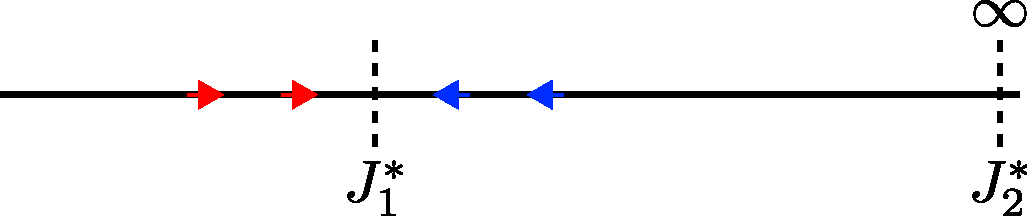
\includegraphics[width=0.49\textwidth]{plt/rg_flow.pdf}
	\caption{The three fixed points of the over-screened RG equation. Only the intermediate one is stable.}
	\label{rg_flow}
\end{figure}

The RG equation reduces to the perturbative form \(\Delta {\mathcal{J}}_{(j)} \simeq \frac{{\mathcal{J}}_{(j)}^2 \mathcal{N}_{(j)}}{D_{(j)}}\left( 1 - \frac{1}{2}\rho {\mathcal{J}}_{(j)} K \right)\)~\cite{Kogan_2018,Kuramoto1998,Noz_blandin_1980,tripathi2018landau} when one replaces \(\omega_{(j)}\) with the ground state energy \(-\frac{D_{(j)}}{2}\) and assumes \({\mathcal{J}} \ll D_{(j)}\).

\subsection{Star graph as the effective fixed point Hamiltonian}
The fixed point Hamiltonian takes the form
\begin{equation}\begin{aligned}
	H^* = \sum_l\left[ \sum^*_{k}\epsilon_{k,l} \hat n_{k\alpha,l} + {\mathcal{J}}\sum_{kk^\prime}^* \vec{S_d}\cdot\frac{1}{2}\vec{\sigma}_{\alpha\alpha^\prime}c_{k\alpha,l}^\dagger c_{k^\prime\alpha^\prime, l}~.\right]
\end{aligned}\end{equation}
We have not explicitly written the decoupled degrees of freedom \(D_{(j)} > D^*\) in the Hamiltonian. The \(*\) over the summations indicate that only the momenta inside the window \(D^*\) enter the summation. There is an implied summation over the spin indices \(\alpha,\beta\).

To study the low energy physics and universality of the problem, we will mostly focus on the zero bandwidth limit of the fixed point Hamiltonian. Upon setting the chemical potential equal to the Fermi energy, this zero bandwidth model becomes a Heisenberg spin-exchange Hamiltonian.
\begin{equation}\begin{aligned}
	\label{stargraph}
	H^* = {\mathcal{J}}\sum_l\sum_{kk^\prime}^* \vec{S_d}\cdot\frac{1}{2}\vec{\sigma}_{\alpha\alpha^\prime}c_{k\alpha,l}^\dagger c_{k^\prime\alpha^\prime, l} = {\mathcal{J}}\vec{S_d}\cdot\vec S~.
\end{aligned}\end{equation}
At the last step, we defined the total bath local spin operator \(S = \sum_l \vec{S}_l = \frac{1}{2}\sigma_l = \frac{1}{2}\sum_{kk^\prime}^*\sum_{\alpha\beta}\vec{\sigma}_{\alpha\alpha^\prime}c_{k\alpha,l}^\dagger c_{k^\prime\alpha^\prime, l}\).
\begin{figure}[htpb]
	\centering
	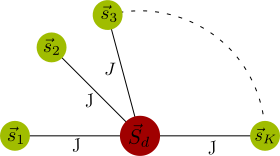
\includegraphics[width=0.30\textwidth]{plt/stargraph.pdf}
	\caption{Zero bandwidth limit of the fixed point Hamiltonian. The central yellow node is the impurity spin, which is talking withe \(K\) green outer nodes that represent the local spins of the channels.}
	\label{fig:stargraph}
\end{figure}
The star graph commutes with several operators, including the total spin operator \(J^z = S_d^z + S^z\) along \(z\), the total bath local spin operator \(S^2\) and the string operators 
\begin{equation}\begin{aligned}
\pi^{x,y,z} = \sigma_d^{x,y,z} \otimes_{l=1}^K \sigma_l^{x,y,z}~.
\end{aligned}\end{equation}
If we define the global spin operator \(\vec J = \vec S + \vec S_d\), the star graph Hamiltonian can be written as \(\mathcal{J}\left[J^2 - S_d^2 - S^2\right] \). The ground state is achieved for the maximal value of \(S\), \(S=\frac{K}{2}\), and the corresponding minimal value of \(J\), \(J = |\frac{K}{2} - S_d|\). This value corresponds to a multiplicity of \(2J+1 = |K - 2S_d|+1\) in \(J^z\), and since the Hamiltonian does not depend on \(J^z\), these orthogonal states \(\ket{J^z}\) constitute a degeneracy of \(g^{S_d}_K = |K - 2S_d|+1\).

The \(\pi^z\) acts on the eigenstates \(\ket{J^z}\) and reveals the odd-even parity of the eigenvalue \(J^z\), and is hence a parity operator. Interestingly, {the string operator \(\pi^z\) is a Wilson loop operator~\cite{fradkin2013field} that wraps around all the nodes of the star graph}:
\begin{equation}\begin{aligned}
	\label{w_loop}
	\pi^z = \exp\left[i \frac{\pi}{2} \left(\sigma_d^z + \sum_{l=1}^K \sigma^z_l - K\right)\right] = e^{i \pi \left(J^z - \frac{1}{2}K\right)}
\end{aligned}\end{equation}
\(\pi^x\) and \(\pi^y\) mix states of opposite parity. For example, it can be shown that \(\pi^x \ket{J^z} = -\ket{J^z}\). These are 't Hooft operators \cite{fradkin2013field}.


There are multiple reasons for working with the star graph in particular and zero mode Hamiltonians in general. In the single-channel Kondo model, the star graph is just the two spin Heisenberg, and it reveals the stabilization of the Kondo model ground state, as well as certain thermodynamic properties (e.g., the impurity contribution to the susceptibility)~\cite{varma_yafet_1976,yosida_1966,wilson1975renormalization,moca_zarand_2021,varma_yafet_1976,kondo_urg}. Similarly in the MCK model, the star graph is able to mimic the nature of the RG flows: At weak coupling \({\mathcal{J}} \to 0^+\), the central spin is weakly coupled to the outer spins and  prone to screening because of the \(S^\pm\) terms in the star graph, and at strong coupling \({\mathcal{J}} \to \infty^-\), the outer spin-half objects tightly bind with the central spin-half object to form a single spin object that interacts with the remaining states through an exchange coupling which is RG relevant, rendering both the terminal fixed points unstable. The true stable fixed point must then lie somewhere in between, and we recover the schematic phase diagram of fig.~\ref{rg_flow}. 

The utility of the star graph is due to the fact that {the non-Fermi liquid arises solely from the degeneracy of the ground state manifold of the underlying zero mode Hamiltonian, and the star graph captures this degeneracy in its entirety}. The RG flows of the MCK model have been show to {preserve the degeneracy of the ground state}~\cite{pang_cox_1991,kroha_kolf_2007,zitko_fabrizio_2017}. The star graph conserves the total spin \(J^z\), and this leads to a ground state degeneracy of \(|K - 2S_d|+1\) in the \(K-\)channel spin-\(S_d\) impurity star graph which is preserved under the RG flow. This is qualitatively different from the case of the single-channel Kondo model where the \(2-\)fold degeneracy of the local moment fixed point crosses over into a stable and unique singlet ground state. 

As we will see in a subsequent section, the lowest excitations of the intermediate fixed point is described a non-Fermi liquid phase induced by nearest-neighbour hopping terms between the zeroth sites and the first sites of the conduction channels. The importance of the degeneracy can be shown in the following manner. As mentioned previously, the ground state degeneracy of the more general star graph with a spin-\({S_d}\) impurity and \(K\) channels is given by \(g^{S_d}_K = |K - 2{S_d}|+1\). The cases of \(K=2{S_d}\), \(K<2{S_d}\) and \(K>2{S_d}\) correspond to exactly screened, under-screened and over-screened regimes respectively. {The latter two cases correspond to a multiply-degenerate manifold \(g^S_K > 1\), and simultaneously have non-Fermi liquid phases~\cite{Noz_blandin_1980,Gan_Andrei_Coleman_1993,emery_kivelson,Gan_mchannel_1994,Tsvelick_Weigmann_mchannel_1984,Tsvelick_weigmann_mchannel_1985,parcollet_olivier_large_N,kimura_taro_Su_N_kondo,PhysRevB.73.224445,cox_jarrell_two_channel_rev,affleck_1991_overscreen,Coleman_tsvelik,affleck1993exact,coleman_pepin_2003,roch_nicolas_costi_2009,schiller_avraham_2008,Durganandini_2011}, while the first regime has a unique ground state \(g^S_K = 1\) and is described by a local Fermi liquid (LFL) phase \cite{wilson1975,nozieres1974fermi,Noz_blandin_1980,andreiKondoreview,tsvelickKondoreview}, thereby substantiating the claim that a degeneracy greater than unity leads to non-Fermi liquid physics.} In the following sections, we will show how the inherent quantum-mechanical frustration of singlet order that is present in the Hamiltonian leads to the degenerate ground state manifold and the non-trivial physics of the fixed points in terms of non-Fermi liquid phase, diverging thermodynamic quantities, quantum criticality as well as emergent gauge theories.
\section{Important Properties of the Star Graph}
\textcolor{red}{\subsection{Hamiltonian and wavefunctions}
\noindent As shown in the previous section, at the heart of multi channel Kondo there is a star graph problem which is the zero mode of the low energy fixed point Hamiltonian of the Multi channel Kondo.In this section our focus will be on the star graph problem itself.
As shown in the Fig.\ref{fig:stargraph} above one central spin ($\vec{S}_d$) is connected with $K$ spins forming a $K$ channel star graph problem corresponding to the $K$-channel Kondo problem. The Hamiltonian of this above model is given as 
\begin{eqnarray}
H &=& {\mathcal{J}} \vec{S}_d.\sum_{i=1}^{K}\vec{S}_i={\mathcal{J}} \vec{S}_d.\vec{S} \nonumber\\
&=& \frac{{\mathcal{J}}}{2} (\vec{J}^2-\vec{S}^2-\vec{S}_d^2)~,~~{\mathcal{J}} >0.
\label{eq:stargraph_hamiltonian}
\end{eqnarray}
where $\vec{J}=\vec{S}+\vec{S}_d$ and $\vec{S}=\sum_{i=1}^{K} \vec{S}_i$. One can see that the large spin $S$ can take many possible values as this is made out of $K$ spin 1/2s. We can see $[H,J]=0=[H,J^i]$ for  $i=x,y,z$, $[J^i,J^j]\neq 0$ for $i\neq j$. In our model we find two string operators $\hat{\mathbb{Z}}=\sigma_d^z\Pi_{i=1}^{K} \sigma_i^z$ and $\hat{\mathbb{X}}=\sigma_d^x\Pi_{i=1}^{K} \sigma_i^x$, where $K$ is the number of channels. These two operators commutes with the Hamiltonian $H$ of this star graph.
\begin{eqnarray}
[H,\hat{\mathbb{Z}}] &=& 0 = [H,\hat{\mathbb{X}}]
\end{eqnarray}
We can rewrite the operators in the form of a twist operator as, $\mathbb{Z}=e^{i\pi [J^z-(\frac{K+1}{2})]}$ and $\mathbb{X}=e^{i\pi [J^x-(\frac{K+1}{2})]}$
The commutation between these two operators are given as
\begin{eqnarray}
[\mathbb{Z},\mathbb{X}] &=& \prod_{i=d,1}^{K} \sigma^z_{i} \prod_{i=d,1}^{K} \sigma^x_{i} \bigg[1-(-1)^{K+1}\bigg]
\end{eqnarray}
\textbf{MERGE THIS WITH EARLIER SUBSECTION.}
Thus we can see that for case where number of channels is odd that means $K+1$ is even, these two string operators commutes with each other forming a CSCO ($H,\hat{\mathbb{Z}},\hat{\mathbb{X}}$). On the other hand in the case where number of channels $K$ is even, these two operators does not commute with each other. Thus we can form the CSCO with $H,J,J^z,S,S_d$. For a particular value $S$, $J$ can take two values $S\pm S_d$ with the energies $-{\mathcal{J}} S_d(S_d+1\mp J)$ respectively. $S_d$ is fixed thus the energy values only depends on the corresponding $J$ value of the state. As the energy does not depends on the $J^z$, all $2J+1$ $J^z$ states labeled by $|S_d,S;J,J^z\rangle$ are degenerate. It is easy to see that the ground state has energy $E=-{\mathcal{J}} S_d(S_d+1+J)$ with  $J=S-S_d$, thus $E_g=-{\mathcal{J}} S_d(S_{max}+1)$ with $S$ taking the maximum possible value $S_{max}=K/2$.
 }

\subsection{Degree of compensation: a measure of the frustration}
One can quantify the amount of screening of the local moment at the impurity site by defining a degree of compensation \(\kappa\). Such a quantity also measures the inherent singlet frustration in the problem: the higher the degree of compensation, the better the spin can be screened into a singlet and lower is the frustration. It is given by the antiferromagnetic correlation existing between the impurity spin and conduction electron channels:
\begin{equation}\begin{aligned}
	\Gamma \equiv - \left< \vec{S_d}\cdot \vec{S}\right>
\end{aligned}\end{equation}
The expectation value is calculated in the ground state. Since the inner product is simply the ground state energy of a spin-\(S\) impurity \(K-\)channel MCK model in units of the exchange coupling \(J\), we have
\begin{equation}\begin{aligned}
	\Gamma = \frac{1}{2} \left[ l_\text{imp}^2 + l_c^2 - g^S_K\left( g^S_K - 1 \right)\right]
\end{aligned}\end{equation}
\(l_\text{imp}^2 = S_d(S_d+1)\) is the length-squared of the impurity spin. Similarly, \(l_c^2 = \frac{K}{2}\left(\frac{K}{2} + 1\right) \) is the length-squared of the total conduction bath spin. \(g^S_K = |K - S_d| + 1\) is the ground state degeneracy. We will explore the three regimes of screening by defining \(K = K_0 + \delta, S = \frac{K_0}{2} - \delta\). \(\delta=0\) represents the exactly-screened case of \(K = 2S = K_0\). Non-zero \(\delta\) represents either over- or under-screening. In terms of \(K_0\) and \(\delta\), the degree of compensation becomes
\begin{equation}\begin{aligned}
	\label{gamma}
	\Gamma = \frac{1}{4}\left[\left( K_0 + 1 \right) ^2 - \left(|\delta| + 1 \right) ^2\right] 
\end{aligned}\end{equation}
{For a given \(K_0\), the degree of compensation is maximised for exact screening \(\delta=0\), and is reduced for \(\delta \neq 0\). This shows the inability of the system to form a unique singlet ground state and reveals the quantum-mechanical frustration inherent in the zero mode Hamiltonian and therefore in the entire problem.} The degree of compensation is symmetric under the Hamiltonian transformation \(\delta \to -\delta\), and this represents a duality transformation between over-screened and under-screened MCK models. This topic will be discussed in more detail later.
\begin{figure}[htpb]
	\centering
	\includegraphics[width=0.49\textwidth]{plt/deg_of_comp.pdf}
	\caption{Variation of the degree of compensation as we tune the system from under-screening to over-screening. The maximum spin compensation occurs at exact-screening \(\delta=0\).}
\end{figure}

\subsection{Impurity magnetization and susceptibility}
In order to obtain the magnetic susceptibility, We insert a magnetic field that acts only on the impurity and then diagonalize the Hamiltonian.
\begin{align}
	\label{stargraph_field_hamiltonian}
	H(h) = {\mathcal{J}^*} \vec{S_d}\cdot\vec{S} + h S_d^z
\end{align}
The Hamiltonian commutes with \(S\), so it is already block-diagonal in terms of the eigenvalues \(M\) of \(S\). \(M\) takes values in the range \(\left[M_\text{min}, M_\text{max}\right]\), where \(M_\text{max} = K/2\) for a \(K-\)channel Kondo model, and \(M_\text{min} = 0\)  if \(K\) is even, otherwise \(\frac{1}{2}\). Defining \(\alpha = \frac{1}{2}\left({\mathcal{J}}m + h\right) + \frac{{\mathcal{J}}}{4}\) and \(x^M_m = M(M+1) - m(m+1)\), the partition function can be written as
\begin{align}
	Z(h) =\sum_{M=M_\text{min}}^{M_\text{max}}r^K_M\left[\sum_{m=-M, \atop{m\in \mathbb{Z}}}^{M-1}2e^{\beta \frac{{\mathcal{J}}}{4}}\cosh \beta\sqrt{{\mathcal{J}}^2x^M_m/4 + \alpha^2} \right.\nonumber\\
\left.+ 2e^{-\beta {\mathcal{J}}M/2}\cosh \beta h/2\right]
\end{align}
Here, \(\beta = \frac{1}{k_B T}\), \(M\) sums over the eigenvalues of \(S\) while \(m\) sums over \({\mathcal{J}}^z - \frac{1}{2}\) and the additional degeneracy factor \(r^K_M= {}^{K-1}C_{K/2 - M}\) arises from the possibility that there are multiple subspaces defined by \(S=M\). 
To calculate the impurity magnetic susceptibility, we will use the expression
\begin{align}
	\chi = \frac{1}{\beta}\lim_{h \to 0}\left[\frac{Z^{\prime\prime}(h)}{Z(h)} - \left(\frac{Z^{\prime}(h)}{Z(h)}\right)^2 \right] 
\end{align}
where the \(\prime\) indicates derivative with respect to \(h\). For brevity, we define \(\theta_M = \beta {\mathcal{J}} (M+\frac{1}{2})/2\) and \(\Sigma_M = \sum_{m=-M, \atop{m\in \mathbb{Z}}}^{M-1}(m+\frac{1}{2})^2\). At low temperatures, the derivatives are 
\begin{align}
	Z &\to 2 r^K_{M_\text{max}} M_\text{max} e^{\beta \frac{J}{2}(M_\text{max} + 1)}\\
	Z^{\prime \prime} &\to r^K_{M_\text{max}}\left(\frac{\beta }{2(M_\text{max} + \frac{1}{2})}\right)^2 e^{\beta \frac{J}{2}(M_\text{max} + 1)}\Sigma_{M_\text{max}}\\
	\chi &\to \frac{\beta\Sigma_\text{max}}{2M_\text{max}\left(2M_\text{max}+1\right)^2} = \frac{\beta(K-1)}{12(K+1)} \sim \frac{1}{T}
\end{align}
\begin{figure}[!htpb]
\centering
\includegraphics[width=0.49\textwidth]{plt/Central_Field_Chi_Powerlaw_}
\caption{Impurity susceptibility vs temperature.}
\label{fig:suseptibility_impurity}
\end{figure}
The susceptibility is plotted in fig.~\ref{fig:suseptibility_impurity}.

This non-analyticity in a response function is a signature of the critical nature of the Hamiltonian. This is in contrast to the behaviour in the non-critical exactly-screened fixed point where the ground state is unique. There, the susceptibility becomes constant at low temperatures: \(\chi(T\to 0) = \frac{W}{4 T_K}\), \(T_K\) being the single-channel Kondo temperature and \(W\) the Wilson number \cite{wilson1975renormalization,nozieres1974fermi,bullaNRGreview,kondo_urg}. We have checked the case of general spin-\(S\) impurity numerically (fig.~\ref{fig:suseptibility_impurity}), and the general conclusion is that all exactly-screened models show a constant impurity susceptibility at \(T \to 0\), while the over-screened and under-screened cases show a diverging impurity susceptibility in the same limit. 

A second non-analyticity arises when we consider the impurity free energy and the magnetization. The thermal free energy is given by
\begin{equation}\begin{aligned}
	F(h) = -\frac{1}{\beta}\ln Z(h) = -\frac{1}{\beta}\ln\sum_{E_n}e^{-\beta E_n}
\end{aligned}\end{equation}
At \(T \to 0\), only the most negative energy \(E_\text{min}\) survives. The minimal energy eigenvalue is
\begin{equation}\begin{aligned}
	E_\text{min} = - \frac{J}{4} - \frac{1}{2}\sqrt{J^2(K+1)^2/4 + h^2 + |h|J(K-1)}
\end{aligned}\end{equation}
The first derivative of the free energy with respect to the field gives
\begin{equation}\begin{aligned}
	F^\prime(h\neq 0, T\to 0) =- \frac{2h + J(K-1)\text{sign}(h)}{4\sqrt{\frac{J^2}{4}(K+1)^2 + h^2 + |h|J(K-1)}}
\end{aligned}\end{equation}
There we used the result that the derivative of \(|x|\) is \(\text{sign}(x)\). If we now take \(h\) to zero from both directions, we get the magnetization of the impurity
\begin{equation}\begin{aligned}
	m = F^\prime(h \to 0^\pm, T\to 0) = \mp \frac{1}{2}\frac{(K-1)}{(K+1)}
\end{aligned}\end{equation}
\begin{figure}[!htpb]
	\centering
	\includegraphics[width=0.49\textwidth]{plt/disc_mag_imp_gen.pdf}
	\caption{Behaviour of the impurity magnetization for three values of \(\left(K, 2S\right) = \left(2, 4\right), \left( 3,3 \right), \left(4, 2\right)  \). Only the case of \(K=2S=3 \left(\delta=0\right)\) is analytic near zero. The non-analyticity of the other cases arises because of the frustration brought about by the degeneracy of the star graph ground state.}
	\label{mag_crit}
\end{figure}

The magnetization is therefore discontinuous as \(h\to 0\); it goes to different values depending on the direction in which we take the limit. The non-analyticity for \(K>1\) occurs because there is at least one pair of ground state with non-zero parity \(\pi^z\) and magnetic field is able to flip one ground state into the state of opposite parity. This available space for scattering is simply the frustration that we discussed earlier. This argument, along with the diverging susceptibility for the over- and under-screened cases, makes it clear that {the non-analyticity and hence the critical nature of the fixed point arise because of the ground state degeneracy, and is therefore a feature of all over-screened and under-screened  models}. Indeed, we have checked numerically (see fig.~\ref{mag_crit}) that the non-analyticity exists for \(\delta \neq 0\), where \(\delta = \frac{K}{2} - S\) is the deviation from exact screening. For \(\delta=0\), the ground state is unique and unfrustrated, so the external magnetic field has no parity-inverted pair to flip across.

\textcolor{red}{Similar study can be done by putting an uniform field on all outer spins and calculating the susceptibility. Here also for all channles $K>2$ the exponent is $-1$ and supports the existence of universality and criticality.
% \begin{figure}[!htpb]
% \centering
% \includegraphics[width=0.49\textwidth]{plt/Outer_Field_Chi_Powerlaw_}
% \caption{Outer susseptibility vs temperature.}
% \label{fig:suseptibility_outer}
% \end{figure}
This susceptibility clearly shown the breakdown of screening in the multichannel cases with degenerate ground states in contrast to the single channel susceptibility which saturates at a finite value at low temperature.}


\subsection{Topological properties of ground state manifold}
\noindent  We can define two operators, for convenience let's call translation and twist operator respectively, $\hat{T}$ and $\hat{O}$ defined as 
\begin{eqnarray}
\hat{T} &=& e^{i\frac{2\pi}{K} \hat{\Sigma}} ~,~\hat{O} = e^{i\hat{\phi}}~,~~\hat{\Sigma}=[\hat{J}^z-(K-1)/2]
\end{eqnarray}
One can see that the generators of these above operators commutes with the Hamiltonian, $[H,J^x]=[H,J^z]=[H,J^z]=0$. In the large channel limit we can do semi-classical approximation. As $J^x$ and $J^y$ both commutes with the Hamiltonian $H$ then $[H,J^y{(J^{x})}^{-1}]=0$, and any non-singular function of these operators must also commute with the Hamiltonian, thus we can say that
\begin{eqnarray}
\hat{\phi}=\tan^{-1}(\hat{J}^y(\hat{J}^x)^{-1})
\end{eqnarray}
Then we get $[\hat{\phi},\hat{H}]=0$. We can label the ground states by the eigenvalues of the translation operator $\hat{T}$. We can also use the ground states labeled by the eigenvalues of $J^z$ ($M$, say). Then the ground states are 
\begin{eqnarray}
|M_1\rangle,|M_2\rangle,|M_2\rangle,\cdots ,|M_K\rangle
\end{eqnarray}
Then the operations of the translation operators on this states are give below.
\begin{eqnarray}
\hat{T}|M_i\rangle &=& e^{i\frac{2\pi}{K} [M_i-(K-1)/2]} |M_i\rangle = e^{i2\pi\frac{p_i}{K} } |M_i\rangle~,~p_i\in[K]~~~~~~~
\end{eqnarray}
Now we check the braiding rule between the twist and the translation operators, we find
\begin{eqnarray}
\hat{T}\hat{O}\hat{T}^{\dagger}\hat{O}^{\dagger} &=& e^{\frac{2\pi }{K}[i\hat{\Sigma},i\hat{\phi}]}=e^{i\frac{2\pi }{K}} \nonumber\\
\hat{T}\hat{O}^m\hat{T}^{\dagger}\hat{O}^{\dagger m} &=& e^{\frac{2\pi }{K}[i\hat{\Sigma},im\hat{\phi}]}=e^{i2\pi \frac{m}{K}}
\end{eqnarray}

Next we shown that the states $\hat{O}^m |M_i\rangle$ are orthogonal to each other and with the state $|M_i\rangle$.

\begin{eqnarray}
\hat{T} \hat{O}^m |M_i\rangle &=& \hat{O}^m \hat{T} e^{i2\pi \frac{m}{K}} |M_i\rangle =\hat{O}^m e^{i \frac{2\pi(m+p_i)}{K} } |M_i\rangle \nonumber\\
\hat{T} \bigg(\hat{O}^m |M_i\rangle \bigg) &=&  e^{i \frac{2\pi(m+p_i)}{K} } \bigg( \hat{O}^m |M_i\rangle \bigg)
\end{eqnarray}
Thus different states $ \hat{O}^m |M_i\rangle$ for different $m$ are labeled by different eigenvalues of the translation operations, thus are orthogonal to each other. Now as the twist operator $\hat{O}$ commutes with the Hamiltonian, thus we can see that 
\begin{eqnarray}
\langle M_i| \hat{O}^{m \dagger}  H \hat{O}^m |M_i\rangle =\langle M_i|  H |M_i\rangle 
\end{eqnarray}
Thus the energy eigenvalues of all the orthogonal states are equal. Thus all the K mutually orthogonal states are degenerate.





\subsection{Local Mott liquid}


\noindent Using the unitary renormalization group method we decouple the impurity spin from the zero-modes of the $K$ channels. We start with the Hamiltonian. The zero mode Hamiltonian is a star graph model 
\begin{eqnarray}
H &=& {\mathcal{J}} \vec{S}_d.\displaystyle\sum_i \vec{S}_i ={\mathcal{J}} S_d^zS^z + \frac{{\mathcal{J}}}{2} (S_d^+S^-+ S_d^-S^+) \nonumber\\
H_D &=& {\mathcal{J}} S^z_d S^z~,~~ H_X = \frac{{\mathcal{J}}}{2} (S_d^+S^-+ S_d^-S^+)
\end{eqnarray}
Here we want to remove the quantum fluctuations between the impurity spin and the rest, for that we do one step URG.
\begin{eqnarray}
\Delta H &=& H_X \frac{1}{\hat{\omega}-H_D} H_X 
\end{eqnarray}
In the zero mode IR fixed point ground state (star graph) of multichannel ground state $J^z$ is a good quantum number but $S^z$ is not. There is no net $S^z$ field thus in the ground state manifold the average $S^z$ is vanishing, $\langle S^z \rangle=0$. We use this expectation value to replace the denominator of the above RG equation.
\begin{eqnarray}
\beta_{\uparrow} ({\mathcal{J}},\omega_{\uparrow})&=& \frac{{\mathcal{J}}^2 \Gamma_{\uparrow}}{2} ~~,~~\Gamma_{\uparrow}=\frac{1}{\omega_{\uparrow}-{\mathcal{J}}(S_d^z-1)}
\end{eqnarray}
Thus we get the effective Hamiltonian is 
\begin{eqnarray}
H_{eff} &=& \frac{{\mathcal{J}}^2 \Gamma_{\uparrow}}{2} (S^2-S^{z2})(\tau^2_{d}-\tau^z_d)  \nonumber\\
%&=& \beta_{\uparrow}(\alpha,\omega_{\uparrow})(S^2-S^{z2})(\tau^2_{d}-\tau^z_d)\\
%~,~~~\frac{\alpha^2 \Gamma_{\uparrow}}{2} =\beta_{\uparrow}(\alpha,\omega_{\uparrow}) \nonumber\\
%&=& \frac{\beta_{\uparrow}(\alpha,\omega_{\uparrow})}{2} (S^2-S^{z2})  \nonumber\\
&& =\frac{\beta_{\uparrow}({\mathcal{J}},\omega_{\uparrow})}{4} (S^+S^-+S^-S^+)   
\end{eqnarray}
In terms of the electronics degree of freedom this looks 
\begin{eqnarray}
%&&H_{eff}(\omega,\alpha)  \nonumber\\
&& \frac{ \beta_{\uparrow}({\mathcal{J}},\omega_{\uparrow}) }{4}   \displaystyle\sum_{\substack{i\neq j \\ \alpha_i,\beta_i\in \{\uparrow,\downarrow\}\\ \alpha_j,\beta_j\in \{\uparrow,\downarrow\}}}\vec{\sigma}_{\alpha_i\beta_i}\vec{\sigma}_{\alpha_j\beta_j}  c_{0\alpha_i}^{(i)\dagger}  c_{0\beta_i}^{(i)}    c_{0\alpha_j}^{(j)\dagger}  c_{0\beta_j}^{(j)} +\textrm{h.c.}   \nonumber
\label{eq:all-to-all_1}
\end{eqnarray}
We will study the two cases of the above effective Hamiltonian depending on the sign of the prefactor. The case $\frac{\beta_{\uparrow}({\mathcal{J}},\omega_{\uparrow})}{2} >0$ is the ferromagnetic case where in the ground state $S$ takes the minimum value and $S^z$ takes the possible maximum value. For an example, in the case of $K$ channels the minimum value of $S$ will be $0$ or $1/2$ for $K$ being $even $ or $odd$ respectively.  We will be interested in the other case where $\frac{\beta_{\uparrow}({\mathcal{J}},\omega_{\uparrow})}{2} <0$. In this case the ground state corresponds to $S$ being maximum and $S^z$ being minimum case. The effective Hamiltonian can be re-written in this case as
\begin{eqnarray}
H_{eff}   =-\frac{|\beta_{\uparrow}({\mathcal{J}},\omega_{\uparrow})|}{4} (S^+S^{-}+ S^-S^{+})    
\end{eqnarray}
\noindent The CSCO of this Hamiltonian contains $H,S,S^z$. In the ground state $S$ is maximum thus $S=K/2$ and $S^z$ can take $2S+1=K+1$ values. Thus in the largest $S$ sector there are $K+1$ states. One can explore different states via a flux tuning mechanism. In the presence of the flux the Hamiltonian looks like \textbf{(SHOW THE BOUNDARY CONDITION CHANGING TWIST OPERATOR THAT LEADS TO THIS FLUX)}
\begin{eqnarray}
H &=& -\frac{|\beta_{\uparrow}({\mathcal{J}},\omega_{\uparrow})|}{2} S^2   +\frac{|\beta_{\uparrow}({\mathcal{J}},\omega_{\uparrow})|}{2} \bigg(S^{z}-\frac{\Phi}{\Phi_0} \bigg)^2 
\label{eq:flux_spectral}
\end{eqnarray}

%\subsubsection{Mapping with the degenerate ground state of stargraph}
\textbf{SHORTEN AND MERGE WITH THE EARLIER SUBSECTION}
\noindent Now we are going to discuss about the mapping of $K$ degenerate ground states of the parent $K-$channel star graph model with the states of this flux-inserted all-to-all model obtained by removing impurity-bath quantum fluctuations. In the star graph model the K ground states is labeled by the $J^z$ eigenvalues. In the star graph ground state $J=S-1/2$, where $S$ is maximum with value $S=K/2$. Thus there are $2J+1=K$ unique $J_z$ eigenvalues corresponding to the $J$ sector labeling different eigenstates. The ground state Hilbert space $\mathcal{H}_{gr}$ contains the $J^z$ states
\begin{eqnarray}
\mathcal{H}_{gr}=\{\textcolor{blue}{-(K-1)/2,-(K-3)/2,\cdots , (K-3)/2,(K-1)/2}\} \nonumber\\
\label{eq:stargraph_states}
\end{eqnarray}
\par Now we shift our focus to the low energy Hamiltonian with flux shown in the eq.\eqref{eq:flux_spectral}. We can see that there is a unique ground state labeled by the $S^z$ eigenvalues. By tuning the flux ($\Phi/\Phi_0$) one can go from one ground state to another ground state or change the ground state. We can see that ground state energy is independent of the configuration of the impurity spin ($S_d^z=\pm 1/2$). Thus for each of those two possibilities we get two set of ground states labeled by the $S^z$ and the $J^z=S^z+S^z_d$. Similar to the star graph case here also the ground state corresponds to the largest $S$ sector, $S=K/2$. Thus total number of $S^z$ eigenvalues are $2S+1=K+1$ taking values $\{ -K/2, -(K-2)/2, \cdots, (K-2)/2, K/2 \}$.
\begin{widetext}
\begin{eqnarray}
S_d^z &=& +1/2~,~ \{J^z\}=\{ \textcolor{blue}{-(K-1)/2, -(K-3)/2, \cdots, (K-1)/2}, (K+1)/2\} \nonumber\\
S_d^z &=& -1/2~,~ \{J^z\}=\{-(K+1)/2,\textcolor{blue}{ -(K-1)/2, \cdots, (K-3)/2, (K-1)/2 } \}
\label{eq:all_to_all_states}
\end{eqnarray}
\end{widetext}

\begin{figure}[!htpb]
\centering
\includegraphics[width=0.49\textwidth]{plt/stargraph-to-alltoall}
\caption{This figure shows the comparison and mapping between the star graph degenerate ground states and the states of the quantum fluctuation resolved all to all model.}
\label{fig:stargraph-to-alltoall}
\end{figure}
Thus one can see that the ground state degeneracy of the star graph model with different $J^z$ values gets lifted in the quantum fluctuation resolved all-to-all model. Depending on the value of the flux there is an unique ground state labeled by the $J^z$ value. Tuning the flux one can go from one ground state to the other. This shows how one can explore different degenerate ground states of the parent star graph model via the insertion of flux in the corresponding quantum fluctuation resolved all-to-all effective Hamiltonian.


\section{Local non-Fermi liquid excitations of the 2-channel Kondo}
\subsection{Effective Hamiltonian}
\textbf{RADICALLY SHORTEN!}
\noindent Here we start with the low energy zero mode fixed point Hamiltonian for the two-channel Kondo obtained under URG treatment. Our goal here is to add excitations on top of this ground state and using the perturbation theory. In doing so we consider the leading order scatter appearing in the lowest order in the perturbative expansion. Note, in the fixed point zero mode Hamiltonian impurity spin is coupled with the bath electrons via spin exchange coupling, there is no charge exchange coupling present. 
\begin{eqnarray}
H^{(2)}&=& {\mathcal{J}} \vec{S}_{imp}.(\vec{S}_1+\vec{S}_2)~~,~~\vec{S}_i =  \frac{1}{2}~ c_{i,\alpha}^{\dagger}~ \vec{\sigma}_{\alpha,\beta}~ c_{i,\beta}
\label{eq:channel-2-spin}
\end{eqnarray}
Here $\vec{S}_i=1,2$ represents the spin degree of freedom present in the origin of the $i^{th}$ channel. Thus one can rewrite the Eq.\eqref{eq:channel-2-spin} in terms of the electronic degree of freedom as,
\begin{eqnarray}
&&\mathcal{H}_0= H_{0_1}+H_{0_2} \nonumber\\
&=&\sum_{i=\{1,2\}}\bigg[ {\mathcal{J}} S^z_{imp}. (n_{i,\uparrow}-n_{i,\downarrow})/2 + \frac{1}{2}  ( S_{imp}^{+} c^{\dagger}_{i,\downarrow} c_{i,\uparrow} + \textrm{h.c.}  )\nonumber \bigg]
\end{eqnarray}
Here the basis we are interested in is $\{\mathcal{B}\}=\{|S^z_{imp},n_{1,\uparrow},n_{1,\downarrow},n_{2,\uparrow},n_{2,\downarrow}\rangle \}$. In this basis we write down all $2^3=8$ states of the spin Hamiltonian eq.\eqref{eq:channel-2-spin}
First the two degenerate ground states with energy $-{\mathcal{J}}= E_{\alpha_0}= E_{\alpha_1}$ is given as,
\begin{eqnarray}
|\alpha_0\rangle &=& \frac{1}{\sqrt{6}} \bigg[2|\Downarrow,1,0,1,0\rangle-|\Uparrow,0,1,1,0\rangle-|\Uparrow,1,0,0,1\rangle\bigg] \nonumber\\
|\alpha_1\rangle &=& \frac{1}{\sqrt{6}} \bigg[2|\Uparrow,0,1,0,1\rangle-|\Downarrow,1,0,0,1\rangle-|\Downarrow,0,1,1,0\rangle\bigg] \nonumber
\end{eqnarray}
The doubly degenerate lowest-lying excited state has energy $E_{\beta_1}=E_{\beta_2}=0$.
\begin{eqnarray}
|\beta_0\rangle &=& \frac{1}{\sqrt{2}}\bigg[|\Downarrow,1,0,0,1\rangle-|\Downarrow,0,1,1,0\rangle \bigg] \nonumber\\
|\beta_1\rangle &=& \frac{1}{\sqrt{2}} \bigg[ |\Uparrow,1,0,0,1\rangle-|\Uparrow,0,1,1,0\rangle \bigg]
\end{eqnarray}
Above these two excited states there are another degenerate excited state manifold with energy $ E_{\gamma_0}=E_{\gamma_1}=E_{\gamma_2}=E_{\gamma_3}=\frac{{\mathcal{J}}}{2}$.
\begin{eqnarray}
|\gamma_{0}\rangle &=&\frac{1}{\sqrt{3}} \bigg[|\Uparrow,0,1,0,1\rangle+|\Downarrow,1,0,0,1\rangle+|\Downarrow,0,1,1,0\rangle \bigg] \nonumber\\
|\gamma_{1}\rangle &=& \frac{1}{\sqrt{3}}\bigg[ |\Uparrow,1,0,0,1\rangle+|\Uparrow,0,1,1,0\rangle+|\Downarrow,1,0,1,0\rangle \bigg] \nonumber\\
|\gamma_{2}\rangle &=& |\Uparrow,1,0,1,0\rangle~,~~|\gamma_{3}\rangle = |\Downarrow,0,1,0,1\rangle 
\end{eqnarray}
Note this spin Hamiltonian has total $8$ states, where ground state is double degenerate with energy $-{\mathcal{J}}$ and the lowest excited state with energy $0$ is also double degenerate and the second excited state with energy ${\mathcal{J}}/2$ is 4-fold degenerate. 
\par On top of the zero mode spin-channel interactions we want to consider the effect of the momentum space kinetic energy term $\sum_{k}\epsilon_k (n_{1,k}+n_{2,k})$. We assume identical dispersion for both the channels. Our zero mode spin Hamiltonian is written in the real space, thus it will be easier to do the perturbation theory on the real space. The Fourier transformation of the momentum space kinetic energy  term leads to real space hopping term. For simplicity we will be considering only nearest neighbor hopping between sites within each channels. The real space hopping contribution to the Hamiltonian $H_X$ with the hooping strength is 
\begin{eqnarray}
H_{X} &=& -t \displaystyle\sum_{\substack{<1,l_1> \\ <2,l_2>}} (c^{\dagger}_{1,\sigma}c_{l_1,\sigma}+c^{\dagger}_{2,\sigma}c_{l_2,\sigma}+ ~\textrm{h.c.})
\end{eqnarray}
Here $l_i$ represents the nearest site to the origin of the $i^{th}$ channel. Thus here we are interested in studying the Hamiltonian $\mathcal{H}_0+H_X$. The perturbation $H_x$ contains scattering which takes the states of the zero mode Hamiltonian out of spin-channel scattering space. Thus before we start the perturbation theory we must expand the basis of the zero mode Hamiltonian itself. Thus the basis which contains the nearest neighbor sites of both the channels is given as 
\begin{eqnarray}
&&\{\mathcal{B}_{extnd}\} \equiv  \{\mathcal{B}\} \otimes  \{|n_{l_1,\uparrow},n_{l_1,\downarrow},n_{l_2,\uparrow},n_{l_2,\downarrow}\rangle\} \\
&=& \{|S^z_{imp},n_{1,\uparrow},n_{1,\downarrow},n_{2,\uparrow},n_{2,\downarrow}\rangle \otimes |n_{l_1,\uparrow},n_{l_1,\downarrow},n_{l_2,\uparrow},n_{l_2,\downarrow}\rangle\} \nonumber
\end{eqnarray}
Note there are $2^4=16$ elements in the subspace $\{|n_{l_1,\uparrow},n_{l_1,\downarrow},n_{l_2,\uparrow},n_{l_2,\downarrow}\rangle\}$. In the spin-channel basis $\{\mathcal{B}\}$ there $2$ degenerate ground states. Because the unperturbed Hamiltonian $\mathcal{H}_0$ has no scattering terms outside the spin sector, in the extended basis $\{\mathcal{B}_{extnd}\}$ the total ground state degeneracy becomes simply $2\times 2^4$, $32$ fold. Thus the total Hamiltonian we are interested in is 
\begin{eqnarray}
\mathcal{H} &=& \frac{{\mathcal{J}}\hbar}{2}~ \vec{S}_d. \displaystyle\sum_{i=\{1,2\}} \displaystyle\sum_{\alpha,\beta\in\{\uparrow,\downarrow\}}c_{i\alpha}^{\dagger} \vec{\sigma}_{\alpha\beta} c_{i\alpha} +H_X
%-t\displaystyle\sum_{i=\{1,2\}}\displaystyle\sum_{\substack{\langle i,l_i \rangle\\ \sigma}}(c^{\dagger}_{i,\sigma} c_{l_i,\sigma}+ \textrm{h.c.}) 
%\\
%&=& \displaystyle\sum_{i=1,2} \bigg[ \alpha\hbar~ \vec{S}_d. \vec{S}_i -t\displaystyle\sum_{\substack{\langle i,l_i \rangle\\ \sigma}}(c^{\dagger}_{i,\sigma} c_{l_i,\sigma}+ \textrm{h.c.}) \bigg] \nonumber\\
%&=& \mathcal{H}_0+H_X
\label{eq:excitation_hamiltonian}
\end{eqnarray}
There are two degenerate states $|\alpha_1\rangle$ and $|\alpha_2\rangle$. Thus the two degenerate ground states in the above basis is give as,
\begin{eqnarray}
|\tilde{\alpha}_0\rangle &=&| {\alpha}_0\rangle\otimes |n_{l_1,\uparrow},n_{l_1,\downarrow},n_{l_2,\uparrow},n_{l_2,\downarrow}\rangle \\
|\tilde{\alpha}_1\rangle &=& | {\alpha}_1\rangle\otimes |n_{l_1,\uparrow},n_{l_1,\downarrow},n_{l_2,\uparrow},n_{l_2,\downarrow}\rangle
\end{eqnarray}
Using degenerate perturbation theory we calculate the first and the second order corrections to the Hamiltonian. The first order and the second order low energy effective Hamiltonian is given as 
\begin{eqnarray}
H^{(1)} &=& \sum_{ij} |\alpha_i\rangle \langle \alpha_i  | V| \alpha_j \rangle \langle \alpha_j |~\nonumber\\
H^{(2)} &=& \sum_{ij} \sum_l |\alpha_i\rangle \frac{\langle \alpha_i  | V| \mu_l \rangle \langle \mu_l  | V| \alpha_j \rangle}{E_0-E_{l}}\langle \alpha_j |
\end{eqnarray}
where $|\alpha_i\rangle$ represents the ground states with energy $E_0$ and $\mu_l$ represents the excited states with energy $E_l$. One can easily check the diagonal term in effective Hamiltonian coming from the $1^{st}$ or any $odd$ order correction is zero as the state never returns to the original starting state via odd number of scatterings. For the case of first order it is easy to see that the off-diagonal correction to the effective Hamiltonian is also zero. Thus the lowest order where we expect the non-zero corrections is the second order. We first calculate the diagonal correction in the first order
\begin{eqnarray}
H^{(2)}_{diag} &=& \sum_{i} \sum_l |\alpha_i\rangle\langle \alpha_i | \frac{|\langle \alpha_i  | V| \mu_l \rangle|^2 }{E_0-E_{l}}
\end{eqnarray}
As single scattering always takes the state outside of the spin-channel, the state $V|\alpha_i\rangle$ is an excited state with energy $0$ ($=E_l$). This $\alpha_i$ representing the ground state can take total $32$ configurations as discussed. Out of this $32$ states $| {\alpha}_0\rangle\otimes |n_{l_1,\uparrow},n_{l_1,\downarrow},n_{l_2,\uparrow},n_{l_2,\downarrow}\rangle$ can take $16$ configurations and $| {\alpha}_1\rangle\otimes |n_{l_1,\uparrow},n_{l_1,\downarrow},n_{l_2,\uparrow},n_{l_2,\downarrow}\rangle$ can take the rest 16 configurations. Note the two degenerate states $|\tilde{\alpha}_0\rangle$  and $|\tilde{\alpha}_1\rangle$ is labeled by the $J^z$ eigenvalue $\pm 1/2$ respectively, where $J^z$ is the total z-component of the impurity and zero modes of the baths. Thus these $32$ ground states can be separated in two 16 state groups labeled by the $J^z=\pm 1/2$ eigenvalues. For the $J^z=1/2$ sector we get the effective Hamiltonian
\begin{eqnarray}
H^{(2)}_{diag} (1/2) &=& \frac{2t^2}{E_0} \hat{I} - \frac{2t^2}{3E_0} ( S_{l_1}^z + S_{l_2}^z)
\end{eqnarray}
Similarly the for $J^z=-1/2$ we get 
\begin{eqnarray}
H^{(2)}_{diag} (-1/2) &=& \frac{2t^2}{E_0} \hat{I} + \frac{2t^2}{3E_0} (S_{l_1}^z+S_{l_2}^z)
%= \frac{2t^2}{E_0} \hat{I} + \frac{4t^2}{3E_0} \bigg[S_{l_1}^z+S_{l_2}^z\bigg]
\end{eqnarray}
where $S_{l_i}^z=(n_{l_i\uparrow}-n_{l_i\downarrow})/2.$ This above result shows that the diagonal correlation to the LEH coming from the ground states $J^z=\pm 1/2$ has a emergent field term. 
\begin{eqnarray}
H^{(2)}_{diag} &=& -4t^2 \hat{I}
\end{eqnarray}
But the total contribution shows the trivial nature of the diagonal part in the LEH. This clearly shown that there is no Fermi liquid terms present in low energy in the 2-channel Kondo problem. Here, $\hat{I}$ is the identity operator made out of all $2^4=16$ possible number operator combinations as shown below
\begin{eqnarray}
\hat{I} &=& \sum_{\hat{o}=\hat{n},(1-\hat{n})} \hat{o}_{l_1,\uparrow}\hat{o}_{l_1,\downarrow} \hat{o}_{l_2,\uparrow}\hat{o}_{l_2,\downarrow}
\end{eqnarray}
Due to the ground state degeneracy in the 2-channel problem, there are possible quantum scattering within the ground state manifold among those degenerate states. This leads to a low energy effective Hamiltonian which is off-diagonal in nature as shown below,
\begin{eqnarray}
H_{NFL}&=&H^{(2)}_{off} = \sum_{i\neq j} \sum_l |\alpha_i\rangle \frac{\langle \alpha_i  | V| \mu_l \rangle \langle \mu_l  | V| \alpha_j \rangle}{E_0-E_{l}}\langle \alpha_j | \nonumber\\
&=& -\frac{8t^2}{3} [ (S_1^z)^2 c_{2\uparrow}^{\dagger}c_{2\downarrow}  (  c_{l_1\uparrow}c_{l_1\downarrow}^{\dagger} +  c_{l_2\uparrow}c_{l_2\downarrow}^{\dagger}  ) \nonumber\\
&+& (S_2^z)^2 c_{1\uparrow}^{\dagger}c_{1\downarrow}  (  c_{l_1\uparrow}c_{l_1\downarrow}^{\dagger} +  c_{l_2\uparrow}c_{l_2\downarrow}^{\dagger}  ) ] + \textrm{h.c.} ~,~~~~
\label{eq:hamiltonian_NFL}
\end{eqnarray}
This LEH is purely a non-Fermi liquid. The emergence of non-Fermi liquid is primarily coming due to the degenerate ground states present in the star graph problem in the absence of the real space hopping terms. One can see that though there was no prior inter channel direct interactions, the LEH shows the emergence of such terms through correlated quantum scatterings. \textbf{MENTION THAT WE HAVE COMPUTED VARIOUS THERMODYNAMIC QUANTITIES THAT ARE IN FAIR AGREEMENT WITH THE LITERATURE. AND THAT THESE ARE SHOWN IN THE SUPPLEMENTARY MATERIALS. ALSO MENTION THAT WE HAVE ALSO DERIVED AN EFFECTIVE HAMILTONIAN FOR THE THREE CHANNEL CASE, ALSO SHOWN IN SUPPLEMENTARY MATERIALS.}


\subsection{Local Marginal Fermi liquid and Orthogonality catastrophe}
The real space local low energy Hamiltonian that takes into account the excitations above the ground state is given by eq.~\ref{eq:hamiltonian_NFL} and can be written as
\begin{equation}\begin{aligned}
	\label{nfl_terms}
	V_\text{eff} = \frac{2t^2}{{\mathcal{J}^*}}\left[\left(\sigma^z_{0,1}\right)^2 s^+_{0,2} + \left(\sigma^z_{0,2}\right)^2 s^+_{0,1}\right] \left(s^-_{1,1} + s^-_{1,2}\right) + \text{h.c.}
\end{aligned}\end{equation}
where \(\sigma^z_{0,l} = \hat n_{0\uparrow,l} - \hat n_{0\downarrow,l}, s^+ = c^\dagger_{0 \uparrow,l}c_{0 \downarrow,l}\) and \(s^- = \left(s^+\right)^\dagger\). The notation \(0\sigma,l\) has the site index \(i=0,1,2,\ldots\) as the first label, the spin index \(\sigma=\uparrow,\downarrow\) as the second label and the channel index \(l=1,2\) as the third index.

These are the terms that are generated because of the presence of the impurity. Such a non-Fermi liquid (NFL) contribution to the effective Hamiltonian and the absence of any Fermi-liquid term at the same order should be contrasted with the local Fermi liquid excitations induced by the singlet ground state of the single-channel Kondo model~\cite{nozieres1974fermi,wilson1975renormalization,hewson1993}. 

We now take the MCK Hamiltonian to strong-coupling, and perform a perturbative treatment of the hopping. At \(J \to \infty\), the perturbative coupling \(t^2/J\) is arbitrarily small and we again obtain Eq.~\ref{nfl_terms}. Such a change from the strong coupling model with parameter \(J\) to a weak coupling model with parameter \(t^2/J\) amounts to a duality transformation~\cite{kroha_kolf_2007,zitko_fabrizio_2017}. It can be shown that the duality transformation leads to an identical MCK model~\cite{kroha_kolf_2007} (self-duality), which implies we can have identical RG flows, and our transformation simply extracts the NFL piece from the dual model. The self-duality also ensures that the critical intermediate-coupling fixed point is unique and can be reached from either of the models.

The diagonal part of eq.~\ref{nfl_terms} is
\begin{equation}\begin{aligned}
	V_\text{eff} = \frac{2t^2}{J}\sum_{l=1,2}\left(\sum_\sigma \hat n_{0\sigma,l}\right) s^+_{0,\bar l}s^-_{1,\bar l} + \text{h.c.}
\end{aligned}\end{equation}
where \(\bar l = 3 - l\) is the channel index complementary to \(l\). We will Fourier transform this effective Hamiltonian into \(k-\)space. The NFL part becomes
\begin{equation}\begin{aligned}
	\label{k_space_od}
	\sum_{\sigma, \left\{k_i,k_i^\prime\right\},l} \frac{2t^2}{J}e^{i\left(k_1 - k_1^\prime\right)a}c^\dagger_{k\sigma,l}c_{k^\prime\sigma,l}c^\dagger_{k_2 \uparrow, \bar l}c_{k_2^\prime \downarrow,\bar l}c^\dagger_{k_1 \downarrow,\bar l}c_{k_1^\prime \uparrow, \bar l} + \text{h.c.} 
\end{aligned}\end{equation}
This form of the Hamiltonian is very similar to the three-particle interaction term in Appendix B of~\cite{anirbanmott1}. The channel indices in Eq.~\ref{k_space_od} can be mapped to the normal directions in~\cite{anirbanmott1}. The 2 particle-1 hole interaction in Eq.~\ref{k_space_od} has a diagonal component which can be obtained by setting \(k=k^\prime, k_1 = k_2^\prime\) and \(k_2 = k_1^\prime\):
\begin{equation}\begin{aligned}
	H_\text{eff,MFL} = \sum_{k, k_1, \atop{k_2,\sigma,  l}} \frac{2t^2e^{i\left(k_1 - k_2\right)a}}{J} \hat n_{k\sigma,l} \hat n_{k_2 \uparrow, \bar l}\left(1 - \hat n_{k_1 \downarrow,\bar l}\right) + \text{h.c.}\\
	= \sum_{k, k_1, \atop{k_2,\sigma,  l}} \frac{4t^2}{J} \cos a\left(k_1 - k_2\right)  \hat n_{k\sigma,l} \hat n_{k_2 \uparrow, \bar l}\left(1 - \hat n_{k_1 \downarrow,\bar l}\right)
\end{aligned}\end{equation}
The most dominant contribution comes from \(k_1 = k_2 = k^\prime\), revealing the non-Fermi liquid metal~\cite{cox_jarrell_two_channel_rev,andrei_jerez_1995}:
\begin{equation}\begin{aligned}
	\label{mfl_large}
	H^*_\text{eff,MFL} = \frac{4t^2}{J} \sum_{\sigma, k, k^\prime, l} \hat n_{k\sigma,l} \hat n_{k^\prime \uparrow, \bar l}\left(1 - \hat n_{k^\prime \downarrow,\bar l}\right)
\end{aligned}\end{equation}
A non-local version of this effective Hamiltonian was found to describe the normal phase of the Mott insulator of the 2D Hubbard model, as seen from a URG analysis~\cite{anirbanmott1,anirbanmott2}. Following~\cite{anirbanmott1}, one can track the RG evolution of the dual coupling \(R_j = \frac{4t^2}{J_j}\) at the \(j^\text{rh}\) RG step, in the form of the URG equation
\begin{equation}\begin{aligned}
	\Delta R_j =- \frac{R_j^2}{\omega - \epsilon_{j}/2 - R_j/8}
\end{aligned}\end{equation}
In the RG equation, \(\epsilon_{j}\) represents the energy of the \(j^\text{th}\) isoenergetic shell. It is seen from the RG equation that \(R\) is relevant in the range of \(\omega < \frac{1}{2}\epsilon_j\) that has been used throughout, leading to a fixed-point at \(R^*/8 = \omega - \frac{1}{2}\epsilon^*)\). The relevance of \(R\) is expected because the strong coupling \(J\) is irrelevant and \(R \sim 1/J\).

The renormalisation in \(R\) leads to a renormalisation in the single-particle self-energy~\cite{anirbanmott1}. The \(k-\)space-averaged self-energy renormalisation is
\begin{equation}\begin{aligned}
	\Delta \Sigma(\omega) = \rho {R^*}^2\int_0^{\epsilon^*} \frac{d\epsilon_j}{\omega - \epsilon_j/2 + R_j/8}
\end{aligned}\end{equation}
The density of states can be approximated to be \(N^*/R^*\), where \(N^*\) is the total number of states over the interval \(R^*\). As suggested by the fixed point value of \(R_j\), we can approximate its behaviour near the fixed point by a linear dependence of the dispersion \(\epsilon_j\). The two limits of the integration are the start and end points of the RG. We start the RG very close to the Fermi surface and move towards the fixed point \(\epsilon^*\). Near the start point, we substitute \(\epsilon = 0\) and \(R = \omega\), following the fixed point condition. From the fixed point condition, we also substitute \(R^*/8 = \omega - \frac{1}{2}\epsilon^*\). On defining \(\bar \omega = N^* \left(\omega - \frac{1}{2}\epsilon^*\right)\), we can write
\begin{equation}\begin{aligned}
	\label{self_energy}
	\Delta \Sigma(\omega) \sim  \bar \omega \ln \frac{N^* \omega}{\bar \omega}
\end{aligned}\end{equation}
The self-energy also provides the quasiparticle residue for each channel\cite{anirbanmott1}:
\begin{equation}\begin{aligned}
	Z(\bar\omega) = \left(2 - \ln \frac{2\bar\omega}{N^* \omega}\right) ^{-1}
\end{aligned}\end{equation}
{As the energy scale \(\omega \to 0\), the \(Z\) vanishes, implying that the ground state and lowest-lying excitations, in the presence of the NFL terms, are not adiabatically connected to the Fermi gas. This is the orthogonality catastrophe~\cite{varma2002singular,anderson_infraredcat,yamada_catastrophe,yamada1979orthogonality} in the two-channel Kondo problem, and it is brought about by the presence of the terms in Eq.~\ref{mfl_large}}. Such terms were absent in the single-channel Kondo model, because there was no multiply-degenerate ground state manifold that allowed scattering. This line of argument shows that the extra degeneracy of the ground state subspace and the frustration of the singlet order that comes about when one upgrades from the single-channel Kondo model to the MCK models is at the heart of the NFL behaviour, and the orthogonality catastrophe should be a general feature of all such frustrated MCK models. A local NFL term was also obtained by Coleman, et al.~\cite{Coleman_tsvelik} in terms of Majorana fermions at the zeroth site and the first site of the \(\sigma-\tau\) version of the two-channel Kondo model. There, they computed a self-energy of the form in eq.~\ref{self_energy}. The common features show the universality between the two-channel Kondo and the \(\sigma-\tau\) models. 

\section{Entanglement properties}
\textbf{MINIMISE THE WORDS RADICALLY!}
\subsection{Entanglement properties of the star graph}
\noindent Using the above exact wavefunctions we can numerically compute various entanglement properties of this star graph model. 

\subsubsection{Impurity entanglement entropy}
\begin{figure}[!htpb]
\centering
\includegraphics[width=0.49\textwidth]{plt/EE_multi_channel_ANN.png}
\caption{Caption }
\label{fig:EE_d}
\end{figure}
\noindent Here we are interested in finding the entanglement of the central impurity spin with the rest of the multichannel bath zero mode. For single channel case the ground state is unique and is $|J=0,J_z=0 \rangle = \frac{1}{\sqrt{2}} (|\uparrow_{d}\downarrow_0\rangle -|\downarrow_d \uparrow_0\rangle)$. Thus, one can easily calculate the reduced density matrix of the impurity by tracing out the $0^{th}$ state. From that reduced density matrix the entanglement entropy is $\log 2$, which is maximum possible for a spin-1/2. In the case of multichannel problem there are $K$ orthogonal set of ground states $|J^z\rangle$, for each such state the entanglement is different. The state $|J^z\rangle \equiv |S_d=1/2,S=K/2;(S-1/2),J^z\rangle$ can be written in the fundamental basis. 
Then the density matrix is $\rho=|J^z\rangle\langle J^z|$ from which we can calculate the reduced density matrix by partial tracing the impurity degree of freedom 
%$\rho_{d}=\textrm{Tr}_{d} \rho=\sum_{S_d^z} \langle S_d^z| \rho | S^z_d\rangle$. 
\begin{eqnarray}
\rho_{d}&=& \textrm{Tr}_{d} \rho=\sum_{S_d^z} \langle S_d^z| \rho | S^z_d\rangle ~,~~EE_d = -\rho_{d} \log \rho_{d}~~~
\end{eqnarray}
\noindent The eigenvalues of this reduced density matrix given by $\lambda_i$ is called entanglement spectrum. We are interested in the von-Neumann entanglement entropy of the impurity spin with the rest ($EE_d$). We are interested in the scaling of this entanglement entropy with the channel number. As shown in the Fig.\ref{fig:EE_d} the x-axis is the channel number and for a particular channel there are may possible entanglement values corresponding to different $J^z$ states. The minimum entanglement entropy state (associated with the $J^z=J$ state) decreases show the classical nature of this maximally polarized state. On the other hand the maximum entanglement entropy (associated with $J^z_{min}$ state) for a particular channel $K$ is saturating to $\log K$ in the large $K$ limit. Another important result that we see, for any odd value of $K$ the minimum entanglement entropy associated with $J^z=0$ is $\log 2$ shows a formation of perfectly entangled state made out of more than 2 spins (e.g; singlet). In this state $|J^z=0\rangle$ all the $K$(odd) outer spins participate in quantum scattering with the central impurity spin in such a way the central spin is maximally entangled which is not the case for any other $J^z$ state. In the large $K$ limit irrespective it's even and odd nature there are always a $J^z_{min}$ state where the central impurity spin is maximally entangled.
\begin{figure}[!htpb]
\centering
\includegraphics[width=0.49\textwidth]{plt/outer_EE_multi_channel_ANN.png}
\caption{caption}
\label{fig:EE_outer}
\end{figure}
In a $K$ channel system all the outer spins are equivalent (has $Z_N$ symmetry), thus studying the entanglement of any one outer spin with the rest is enough. Here we do a similar entanglement entropy study where we get the reduced density matrix ($\rho_o$) by partial tracing out any one outer spin say the $l^{th}$ ($1\leq l \leq K$) one $S^z_{l}$. 
\begin{eqnarray}
\rho_{o} &=& \textrm{Tr}_{l} \rho =\displaystyle\sum_{S^z_{l}} \langle S^z_l | \rho | S^z_{l} \rangle~,~EE_o=-\rho_{o}\log \rho_{o}
\end{eqnarray}
We do a similar entanglement scaling with the channel number $K$. We find that minimum entanglement entropy associated with the state $J^z=J$ is approaching zero in the limit $K\gg 1$. In contrast the minimum entanglement entropy associated with $J^z_{min}$ state is saturating at $\log 2$ in the large $K$. Thus in the state $J^z=0$ for any $K$ (or $J^z=\pm 1/2$ for $K\gg 1$) any outer spin is maximally entangled with the rest.

\par The above entanglement studies Fig.(\ref{fig:EE_d},\ref{fig:EE_outer}) show  that for odd channel case there exist a state $J^z=0$ where the central spin $S_d$ and any outer spin $S_i$ is maximally entangled with the rest. This shows the special and unique property of the star graph ground state where you can create state made out of more than 2 spins where each any every one is maximally entangled with the rest. Thus this star graph ground state is very important in the quantum information theory. 

\subsubsection{Mutual Information}

\begin{figure}[!htpb]
\includegraphics[width=0.49\textwidth]{plt/NEW31Dec_I_2_vs_Nch_[0,1]}
\caption{ds}
\label{fig:MI_d_o}
\end{figure}
\noindent In the above study our focus was on the von-Neumann entanglement entropy, now we are interested in the correlation signatures present in the star graph grounds states. Mutual information is one such measure which captures the correlations present between two subsystems (A,B) in a particular state defined as
\begin{eqnarray}
I^2(A:B)=S_A+S_B-S_{A\cup B}
\end{eqnarray}
where $S_{A}$ is the von-Neumann entanglement entropy of the subsystem $A$ with the rest. Here we are interested in computing two types of mutual information first, study the mutual information between the impurity-spin and one outer spin $I^2(d:o)$. Because all the outer spins are symmetric, the mutual information between impurity-spin with any one outer spin is same and can capture the correlation between two $A$ and $B$. We have done a scaling study of this mutual information for different channel numbers $K$. As shown in the Fig.\ref{fig:MI_d_o} in the large $K$ limit the maximum of the mutual information associated with the state $J^z_{min}$ is saturating at $0.3748$ and the Mutual information associated with the state $J^z=J$ is decreasing showing the classical limit.
\begin{figure}[!htpb]
\includegraphics[width=0.49\textwidth]{plt/NEW31Dec_I_2_vs_Nch_[1,2]}
\caption{ds}
\label{fig:MI_o_o}
\end{figure}
Next, we have done a similar study by calculating the mutual information between two outer spin $I^2(o:o)$. In this also we find that the maximum mutual information between any outer spins saturates at the value $0.3759$ very close to the $I^2(d:o)$ case.

\par As can be seen from the above Figure.(\ref{fig:MI_d_o},\ref{fig:MI_o_o}) that  both the maximum mutual information of $I^2(d:o)$ and $I^2(o:o)$ try to saturate near the same value. Thus in the large $K$ limit in the $J^z_{min}$ state mutual information between any two spins in the star graph model is same saturating at a constant value ($0.37$). Though the difference can be seen in the state $J^z=J$ where the mutual information thus correlation s between two outer spins vanishes in the large $K$ limit faster than the mutual information between the impurity and any one outer spin. Thus correlation wise there is no difference between impurity-outer pair and outer-outer pair in the large $K$ limit.


\subsubsection{Multipartite information}
\noindent Similar to the mutual information one can calculate any higher order multipartite information to find the nature of the correlations present in different ground states. We define the tripartite information among three subsystems $A,B,C$ as $I^3_{ABC} = (S_A+S_B+S_C)-(S_{AB}+S_{BC}+S_{CA})+S_{ABC}~$. This tripartite information scaling with the number of channels $K$ also shown behavior similar to the mutual information case, the highest tripartite information is associated with the $J^z_{min}$ state and saturating in the limit of $K\gg 1$. One can measure $N-$partite information for a collection of subsystems (CSS) $\{\mathcal{A}\}\equiv\{A_1,A_2,\cdots,A_K\}$. To define the $N-$partite information, we first define the power set of the CSS $\{\mathcal{A}_N\}$ as $\mathcal{P}(\{\mathcal{A}_{N}\})$, and the collection of all subsets of $\mathcal{P}(\{\mathcal{A}_{N}\})$ with $m$ subsystems in it as $\mathcal{B}_m(\{\mathcal{A}_N\})\equiv \{ Q~| ~Q\subset \mathcal{P}(\{\mathcal{A}_{N}\}), |Q|=m \}$. We also define the union and intersection of all the subsystems present in $Q$ as ${V}_{\cup}({Q})\equiv \bigcup_{A\in Q} A$ and ${V}_{\cap}({Q})\equiv \bigcap_{A\in Q} A$ respectively. Finally, the von Neumann entanglement entropy of the subsystem $A$ is given by $S_{A} $. Then the $N-$partite information that we are interested in is defined as
\begin{eqnarray}
I^{N}_{\{\mathcal{A}_N\}} &=& \bigg[\displaystyle\sum_{m=1}^{N} (-1)^{m-1} \displaystyle\sum_{Q \in \mathcal{B}_m(\{\mathcal{A}\})} S_{V_{\cup}({Q})} \bigg]- S_{V_{\cap}(\mathcal{A}_N)}~.~~~~
\label{eq:I_N_definition}
\end{eqnarray}
Studying these multipartite information one can understand the nature of the correlations present among the outer spins.
\begin{figure}
\includegraphics[width=0.49\textwidth]{plt/IN_vs_N_K8.png}
%I_N_vs_N_N9.png}
\caption{This figure shows how the $m-partite$ information varies with $m$ showing the entanglement distribution among different number of outer-spins.}
\label{fig:Im_vs_m}
\end{figure}
\noindent Our study of this multi-partite information presented in the above Fig.\eqref{fig:Im_vs_m} shows that the higher oreder multi partite information decreases as you increase the order following a power law.





\subsection{Entanglement properties of the multichannel Kondo fixed point}
\begin{figure}[!htpb]
\includegraphics[width=0.49\textwidth]{plt/hopping_fock_states}
\caption{This is a schematic diagram of (a) single channel and (b) two channel problem. $S_d$ is the impurity spin. For more details refer to the text.}
\label{fig:schematic_hopping}
\end{figure}


\noindent Apart from various thermodynamic properties of the local NFL, here we study the various entanglement signatures present in the ground state. We start with the Hamiltonian Eq.\eqref{eq:excitation_hamiltonian} where we are only taking the nearest neighbor real space hopping (t) where $t=0$ case is the zero mode Hamiltonian of the multichannel Kondo as shown in the Fig.\ref{fig:schematic_hopping}. In the single channel case the impurity ($S_d$) is talking to the spin degree of freedom at the real space origin ($\{1_{\uparrow},1_{\downarrow}\}$) of the unique conduction bath via a Heisenberg coupling. For $2$ channel case the impurity is talking to $2$ different origins of different conduction channels ($\{1_{\uparrow},1_{\downarrow}\}$ and $\{2_{\uparrow},2_{\downarrow}\}$) and hopping connects to their nearest neighbor sites, for example $\{1_{\uparrow},1_{\downarrow}\}$ connects to $\{l_{1\uparrow},l_{1\downarrow}\}$. Thus, for $K$ channel case we are solving a problem with one spin 1/2 degree of freedom and $2K$ electronic sites. As we increase the hopping strength $t$ from zero to non-zero, the sites of the zero mode Hamiltonian starts to scatter with their respective nearest neighbor sites.


\begin{figure}[!htpb]
\centering
\includegraphics[width=0.49\textwidth]{plt/A_I1_ch123_['d']}
\includegraphics[width=0.49\textwidth]{plt/errorbar_A_I1_ch123_['d']}
%\includegraphics[width=0.49\textwidth]{plt/EE_imp_vs_t_K=12}
\caption{This Figures shown the variation of impurity entanglement entropy $EE_{imp}$ with the variation of the hopping strangth $t$ for three different channel cases, $K=1,2,3$. In this case we have fixed $\alpha=1$.}
\label{fig:EE_imp_vs_t_K}
\end{figure}

\subsubsection{Impurity entanglement entropy}
\noindent  First, we are interested in the impurity entanglement entropy which is a measure of entanglement of the impurity with the rest. To do so we calculate the ground state of the Hamiltonian Eq.\eqref{eq:excitation_hamiltonian} $|\psi_g(t)\rangle$ followed by density matrix $\rho_g(t)=|\psi_g(t)\rangle \langle\psi_g (t)|$. Then we calculate the reduced density matrix by partial tracing the impurity $\rho_{imp}(t)=Tr_{imp} \rho_g(t)$. By diagonalizing the reduced density matrix $\rho_{imp}(t)$ we get the eigenvalues $\lambda_i(t)$ and the von-Neumann entanglement entropy $EE_{imp}(t)=-\sum_i\lambda_i(t) \log \lambda_i(t)$. As shown in the Fig.\ref{fig:EE_imp_vs_t_K} for all the three channel cases at low hopping strength $t$ there is a plateau in the $EE_{imp}$ measurement before it starts to decline with the further increase of hopping strength. At low $t\ll 1$ single channel has the higher impurity entanglement, which decreases by the increase of the channel number. On the other hand at high hopping strength value we see a different ordering of the impurity entanglement entropy. Higher the channel number slower the fall of the $EE_{imp}$ with the increase of $t$. This shows that, multiple channels protects the impurity better in terms of impurity  entanglement entropy making the multi channel problem more robust against the single channel case. 
\par Though the plateau value of the impurity entanglement entropy at low hopping strength is very close to each other for different channel cases, there is a distinct difference between them. For the single channel case, the impurity entanglement entropy varies smoothly with the increase of $t$ from zero to nonzero value without any discontinuity. On the other hand for higher channels like $K=2$ and $K=3$ there is a discontinuity in the impurity entanglement entropy at $t=0^+$.


\begin{figure}[!htpb]
\includegraphics[width=0.49\textwidth]{plt/A_I2_ch12_['d','1_up']}
\includegraphics[width=0.49\textwidth]{plt/errorbar_A_I2_ch12_['d','1_up']}
\caption{This figure show the variation of mutual information between the impurity spin and $1_{\uparrow}$ state with respect to the variation of the hopping strength $t$. For more details please refer to the text. In the figure above $\gamma=0.2195$.}
\label{fig:MI_imp_1_vs_t_K}
\end{figure}

\subsubsection{Intra-channel Mutual information}

\noindent Here we are interested in calculating Mutual information between two Fock states in the ground state wavefunction as a function of the hopping strength $t$ varying from $0$ to non zero values. Mutual information between two sub-systems $A,B$ is defined as $MI(A:B)=S(A)+S(B)-S(A\cup B)$, where $S(A)$ is the von-Neumann entanglement entropy of the sub-system $A$ with the rest of the system. 

\noindent To find out the entanglement present between two Fock states within a single channel, we calulate the intra-channel mutual information.

\par \textit{Case 1:} First, we study the mutual information between the impurity spin $S_d$ and $1_\uparrow$ Fock state (Fig.\ref{fig:schematic_hopping}) represented as $MI(d,1\uparrow)$, where $1$ is realspace origin of the $1^{st}$ conduction channel. For single channel case this $1_{\uparrow}$ site can be chosen uniquely but for $K$ channel cases there are $K$ possible choices, due to the symmetry any one choice will show similar mutual information signature. Similarly due to the $SU(2)$ spin rotation symmetry the mutual information between the impurity spin and $1_{\downarrow}$ state will not be any different. We have numerically computed the variation of mutual information with respect to the hopping strength $t$ and presented in the Fig.\ref{fig:MI_imp_1_vs_t_K}.  As shown in the inset of the Fig.\ref{fig:MI_imp_1_vs_t_K} at low hopping strength the mutual information for both the single channel and twochannel cases is saturating at different values. In the single channel case the Mutual information for $t=0$ is $MI(d,1_{\uparrow})=\log 2$ and changes smoothly to nozero $t$ values, similar to the previous impurity entanglement entropy study ($EE_{imp}$).
\begin{eqnarray}
S_{d}=S_{1_{\uparrow}}=S_{d,1_{\uparrow}}=\log 2~,~MI(d,1_{\uparrow})=\log 2
\end{eqnarray}
This $\log 2$ value shows the stability of the zero mode of single channel and perfect screening. Next we focus to the two channel case where the mutual information is $MI(d,1_{\uparrow})=0.2401$ which is less than the single channel case showing the breakdown of screening. Note, unlike the single channel case there is a discontinuity in $MI(d,1_{\uparrow})$ at $t=0^+$.



\begin{figure}[!htpb]
\includegraphics[width=0.49\textwidth]{plt/A_I2_ch12_['1_up','1_down']}
\includegraphics[width=0.49\textwidth]{plt/errorbar_A_I2_ch12_['1_up','1_down']}

\caption{This figure shows the variation of mutual information among the two fock states present on the realspace origin of a conduction channel with $t$. In the figure above $\delta=0.490$}
\label{fig:MI_1_2_vs_t_K}
\end{figure}

\par\textit{Case 2:} Similarly we have computed the mutual information $MI(1_{\uparrow},1_{\downarrow})$ (Fig.\ref{fig:MI_1_2_vs_t_K}) which measures intra channel  mutual information beteen two fock states $1_{\uparrow},1_{\downarrow}$ present at realspace origin. We find that the Mutual information is a smooth function of $t$ for single channel and for two channel there is a discontinuity at $t=0^{+}$. Note, $MI(1_{\uparrow},1_{\downarrow})>MI(d,1_{\uparrow})$ for all $t$ values show the presence of stronger intra-site correlation.

\begin{figure}
\includegraphics[width=0.49\textwidth]{plt/A_I2_ch12_['d','l1_up']}
\includegraphics[width=0.49\textwidth]{plt/errorbar_A_I2_ch12_['d','l1_up']}
\caption{$MI(d,l_{1\uparrow})$}
\label{fig:MI_d_l1}
\end{figure}
\par \textit{Case 3:} Here we measure mutual information between the impurity and the Fock state of the nearest neighbor site to the realspace origin (Fig.\ref{fig:schematic_hopping}) of the conduction channel, $MI(d,l_{1\uparrow})$ as shown in the Fig.\ref{fig:MI_d_l1}. Vanishing mutual information for the single channel case shows the perfect screening of the impurity spin. On the other had we expect the breakdown of screening in two channel case, which is confirmed by the non-zero value of mutual information at small $t$ values. Here also we find a dicontinuity inthe mutual information at $t=0^+$.


\begin{figure}[!htpb]
\includegraphics[width=0.49\textwidth]{plt/A_I2_ch12_['1','l1']}
\includegraphics[width=0.49\textwidth]{plt/errorbar_A_I2_ch12_['1','l1']}
\caption{$MI(1_{\sigma},l_{1\sigma})$}
\label{fig:MI_l_l1}
\end{figure}

\par \textit{Case 4:} Another complementary study can be made by measuring the mutual information between conduction channel realspace origin and it's nearest neighbor site to check their mutual entanglement. As shown in the Fig.\ref{fig:MI_l_l1}, we find that at low hopping strength the single channel mutual information vanishes showing the decoupling of those two states. On the other hand in the two channel case there is a nonzero mutual information which verifies the presence of active scattering between the local Mott liquid and the local non-Fermi liquid phases. Similar discontinuity in the mutual information was observed at $t=0^+$.


\par All the above  entanglement studies suggest that for two channel problem there is a discontinuity in the ground state at $t=0^{+}$, whereas for the single channel case it is a smooth function. Thus for single channel case the $t=0$ and $t\neq 0$ cases can be adiabtically connected, which is not the case for any other channel cases. 


\subsubsection{Inter-channel Mutual information}
Apart from the intra-channel mutual information, here we study the mutual information between two channels to calculate the entanglement content within the local Mott liquid phase.
\begin{figure}
\includegraphics[width=0.49\textwidth]{plt/A_I2_ch2_[1,3]}
\includegraphics[width=0.49\textwidth]{plt/errorbar_A_I2_ch2_[1,3]}
\caption{$MI(1_{\sigma},2_{\sigma'})$}
\label{fig:MI_1_2}
\end{figure}
In the Fig.\ref{fig:MI_1_2} above we study the mutual information $MI(1_{\sigma},1_{\sigma'})$ between two Fock states $1_{\sigma},1_{\sigma'}$ as shown in the Fig.\ref{fig:schematic_hopping} for the two channel case. This shows that at low hopping strength there is a non-zero mutual information. This confirms the presence of correlation among channels. Apart from mutual information we have also computed the tripartite information across channels for this two channel case in the presence of non-zero hopping.
\subsubsection{Tripartite information}

\begin{figure}
\includegraphics[width=0.49\textwidth]{plt/A_I3_ch2_[1,5,6]}
\includegraphics[width=0.49\textwidth]{plt/errorbar_A_I3_ch2_[1,5,6]}
\caption{Tripartite information TPI 156}
\label{fig:TPI_1_5_6}
\end{figure}
As shown in the result above Fig.\ref{fig:TPI_1_5_6} the tripartite information has a discontinuity at $t=0^+$. For small $t$ values the presnece of non-zero tripartite information signals the presence of tripartie correltaion in the ground state which agrees with presence of Marginal Fermi liquid phase shown by the effective Hamiltonian study.


\subsubsection{Bures distance and orthogonality catathrope}
\noindent Apart from different entanglement measures we have measured the Bures distance, which is a measure of distance between two density matrices. Which is defined as 
\begin{eqnarray}
d_{Bures}(\rho_1,\rho_2) &=& \sqrt{2} \bigg[1- \textrm{Tr}\bigg\{ \bigg(\rho_1^{1/2}  \rho_2 \rho_{1}^{1/2}\bigg)^{1/2} \bigg\}\bigg]
\end{eqnarray}
One can see from the above defination that, the maximum and minimum distance it can have is $\sqrt{2}$ and $0$ respectively. This measure represents the distance between two states in a Hilbert space. 
\par We get the ground state wavefunction of the problem by solving the Hamiltonian Eq.\eqref{eq:excitation_hamiltonian} $|\psi(t)\rangle$ which is a function of $t$ and $\rho(t)= |\psi(t)\rangle \langle \psi(t)|$. We are interested in the reduced density matrix of the star graph sites, to get that we partial trace out all other nearest neighbor sites, $\rho_{sg}(t)=\textrm{Tr}_{NN}(\rho(t))$. Then the Bures distance between the reduced denisty matrices $\rho_{sg}(t=0)$ and $\rho_{sg}(t)$, denoted as $d_{Bures}(\rho_{sg}(t=0),\rho_{sg}(t))$ are computed for single, two and three channel cases.
\begin{figure}[!htpb]
\includegraphics[width=0.49\textwidth]{plt/error_Bures_Distance_Ch123_10001}
\includegraphics[width=0.49\textwidth]{plt/errorbar_Bures_Distance_Ch123_10001}
\caption{Bures distance}
\label{fig:bures_distance}
\end{figure}
We have shown the variation of the Bures distance as a function of the hopping strength in the Fig.\ref{fig:bures_distance} above. For all three cases the Bures distance is zero at $t=0$, whic is obvious. But as you turn on $t$ slightly there is a discontinuity in the distance for two and theree channel cases against the single channel where the distance varies smoothly. This discontinuity in the higher channel case against the single channel is similar to all the above entanglement studies. The smooth variation of the distance in the single channel case shows the adiabatic continuation of the reduced stargarph density matrix from the $t=0$ case to $t\neq 0$ case. On the other had the abrupt jump in the Bures distance for higher-channel cases at $t=0^+$ shows the breakdown of adiabatic continuity siganling an orthogonality catastrophe. Three channel case show higher amoount of discontinuity than the two channel case saturating at higher value for $t=1$. Due to finite size system we cannot see the exact orthogonality by getting the $d_{Bures}=\sqrt{2}$, but higher channel cases with higher discontinuity suggests so.


\section{Dualities of the multichannel Kondo model}
We start from a strong coupling \((J \to \infty)\) spin-\(S\) impurity MCK Hamiltonian in the over-screened regime \(\left( K > 2S \right) \),
\begin{equation}\begin{aligned}
	\label{strong_ham}
	H(J) = \sum_{k,\sigma,l}\epsilon_{k,l} \hat n_{k\sigma,l} + J \vec{S_d}\cdot\vec{S}~.
\end{aligned}\end{equation}
Here, \(\vec S\) is the total spin \(\sum_l \sum_{kk^\prime \alpha\beta} \vec \sigma_{\alpha\beta}c^\dagger_{k\alpha,l}c_{k^\prime\beta,l}\) of all the zero modes. At strong coupling, the ground states of the star graph eq.~\ref{stargraph} act as a good starting point for a perturbative expansion. As argued previously, there are \(K-2S+1\) ground states, labeled by the \(K\) values of the total spin angular momentum \(S^z = S_d^z + S^z = -\frac{K}{2} + S, -\frac{K}{2} + S + 1, \ldots, \frac{K}{2} - S\). To leverage the large coupling, one can define a new spin impurity \(\mathbb{S}\) out of this ground state manifold. Since the degeneracy of a spin is given by its multiplicity \(2S^\prime + 1\), we have \(2S^\prime + 1 = K-2S+1 \implies S^\prime = \frac{K}{2} - S\). That is, the spin-\(S\) impurity has a dual described by a spin-\((K-2S+1)\) impurity. The states of this new spin are defined by
\begin{gather}
	\mathbb{S}_d^z \ket{S^z} = S^z \ket{S^z},\nonumber\\
	\mathbb{S}_d^\pm \ket{S^z} = \sqrt{S^\prime\left( S^\prime + 1 \right) - S^z\left( S^z \pm 1\right)} \ket{S^z \pm 1}
\end{gather}
The excited states of the star graph can be used to define bosons \cite{kroha_kolf_2007}, and the hopping into the lattice can then be re-written using these Bosons. One can then remove the single-particle hoping between the zero modes and the first sites using a Schrieffer-Wolff transformation in the small coupling \(J^\prime = \gamma \frac{4t^2}{J}\), and generate an exchange-coupling between the new impurity \(\vec {\mathbb{S}}_d\) and the new zero modes formed out of the remaining sites in the lattice \cite{kroha_kolf_2007} (by remaining, we mean those real space sites that have not been consumed into forming the new spin). The new Hamiltonian, characterized by the small super-exchange  coupling \(J^\prime\), has the form
\begin{equation}\begin{aligned}
	H^\prime(J^\prime) = \sum_{k,\sigma,l}\epsilon_{k,l} \hat n_{k\sigma,l} + J^\prime \vec{\mathbb{S}_d}\cdot\vec{S^\prime}
\end{aligned}\end{equation}
The prime on \(S\) indicates that it is formed by the new zero modes. This Hamiltonian is very similar to the one in eq.~\ref{strong_ham}, and that is the essence of the strong-weak duality: One can go from the over-screened strong coupling spin-\(S\) MCK model to another over-screened weak coupling spin-\((K-2S+1)\) MCK model. For the case of \(K=4S\), we have \(S^\prime = S\), and both \(S_d\) and \(\mathbb{S}_d\) describe the same spin objects (at least formally). The two models are then said to be self-dual. For example, for the case of spin-half MCK model, two-channel model is self-dual.
\begin{figure}[!htpb]
	\centering
	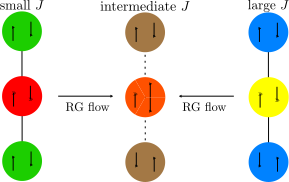
\includegraphics[width=0.3\textwidth]{plt/duality.pdf}
	\caption{Duality of the RG flows as seen in the star graph Hamiltonian. The red and green circles represent the impurity and zeroth site spins respectively. At large \(J\), the red circle binds with the green circles to form an effective spin \(\frac{K-1}{2}\) object (yellow) that interacts with the remaining spin of the conduction bath (blue circles).}
	\label{duality_fig}
\end{figure}

One important consequence of the duality relationship between the two over-screened models is that the RG equations are also dual; while the strong coupling model has an irrelevant coupling \(J\) that flows down to the intermediate fixed point \({\mathcal{J}^*}\), the weak coupling model has a relevant coupling \(J^\prime\) that flows up to the same fixed point \({J^\prime}^* = {\mathcal{J}^*}\). From the RG equation for the general spin-\(S\) MCK model, we know that \({J^\prime}^* = \frac{2}{K \rho^\prime}\), where \(\rho^\prime\) is the DOS for the bath of the weak coupling Hamiltonian. This constrains the form of the scaling factor \(\gamma\):
\begin{equation}\begin{aligned}
	{J^\prime}^* = \frac{\gamma 4t^2}{{\mathcal{J}^*}} = \frac{2}{K \rho^\prime} \implies \gamma = \frac{1}{4t^2} {{\mathcal{J}^*}}^2 = \frac{1}{K^2 t^2 \rho \rho^\prime}
\end{aligned}\end{equation}

There exists another set of dual points in the MCK model. This was hinted at when we looked at the degree of compassion in eq.~\ref{gamma}. Since \(\Gamma\) depends only on the magnitude of \(\delta\), both \(\pm \delta\) will give the same degree of compensation, same ground state energy and same ground state degeneracy \(\left(g^S_K = |\delta|+1\right)\). The definition of \(\delta\) gives the duality transformation as \(K \to 2S, S \to \frac{K}{2}\). That is, we transform from a \(K-\)channel MCK model with spin-\(S\) impurity, to a \(2S\)-channel MCK with a spin-\(\frac{K}{2}\) impurity. The exactly-screened model \(K=2S\) maps on to itself and is therefore self-dual under this transformation.

For \(K \neq 2S\), we transform an over-screened model into an under-screened model and vice versa. This duality relationship allows us to infer the RG scaling behaviour of one of the models if we know that of the other. If we know that for a certain pair of values \(K\) and \(S\), the \(K-\)channel MCK model with spin-\(S\) impurity has an intermediate fixed point, we can immediately conclude that the \(2S\)-channel spin-\(\frac{K}{2}\) model has a strong coupling fixed point.
% \begin{figure}[htpb]
% 	\centering
% 	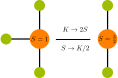
\includegraphics[width=0.3\textwidth]{plt/duality2.pdf}
% 	\caption{Duality between underscreened and overscreened MCK models}
% \end{figure}

\section{Impurity Quantum Phase transition in the multichannel Kondo model under channel anisotropy}
\label{anisotropic_rg}
\textbf{RADICALLY SHORTEN AND RESTRUCTURE THIS SECTION. SHOW THE NUMERICS FIRST, THEN SHOW THE RG 
EQUATION AND QUICKLY DISCUSS ITS CONSEQUENCES.}

\noindent So far we have talked the star graph problem where all the outer spin is coupled with the central impurity spin with Heisenberg coupling of equal strength. This model has a special symmetry where any rearrangement of the outer spins keeps the star graph Hamiltonian invariant. Here we wish to break this symmetry of this Hamiltonian by choosing the individual coupling strength of the outer spin with the central impurity spin different. We start with the general coupling Hamiltonian written as 
\begin{eqnarray}
H_K (\vec{{\mathcal{J}}}) &=& \sum_{i=1}^{K} {\mathcal{J}}_i\vec{S}_d.\vec{S}_i
\label{eq:anisotropy}
\end{eqnarray}

\begin{figure*}
	\centering
\includegraphics[width=0.8\textwidth]{plt/Anisotropy_Channel_3.png}
\caption{[\textbf{CAPTION NEEDED}] channel anisotropy}
\label{fig:channel-anisotropy}
\end{figure*}
where $ \vec{{\mathcal{J}}} \equiv ({\mathcal{J}}_1,\cdots,{\mathcal{J}}_K)$ and ${\mathcal{J}}_i>0, \forall~i$. So far we have considered the case where ${\mathcal{J}}_i={\mathcal{J}},~\forall~i$. Numerical study of the Hamiltonian Eq.\eqref{eq:anisotropy} shown that for any values of coupling ${\mathcal{J}}_i>0$ the ground state degeneracy for a $S_d=1/2$ is always $K$ fold, where $K$ is the number of channels. This shows the robustness of the ground state degeneracy of the star graph model against the coupling anisotropy. The ground state degeneracy only changes when at least one coupling vanishes or becomes infinite. In the case when one coupling of $K$ channel anisotropic star graph model vanishes, the effective model becomes a $K-1$ channel anisotropic star graph model with $K-1$ fold degenerate ground states. On the other hand, if one of the $K$ couplings becomes infinite then with respect to that coupling other couplings becomes zero thus giving rise to an effective single channel star graph model. For example, for ${\mathcal{J}}_K\rightarrow 0$, the Hamiltonian becomes $H_{K}(\vec{{\mathcal{J}}})\rightarrow H_{K-1}({\mathcal{J}}_1,\cdots,{\mathcal{J}}_{K-1})$ and for ${\mathcal{J}}_K\rightarrow \infty$ we get $H_{K}(\vec{{\mathcal{J}}}) \rightarrow H_{1}({\mathcal{J}}_K)$. 

We have demonstrated this numerically for a three channel anisotropic star graph model. As shown in the Fig.\ref{fig:channel-anisotropy}(a) where two couplings are same (${\mathcal{J}}_1={\mathcal{J}}_2=1$) and we are numerically varying the third coupling ${\mathcal{J}}_3$ from finite to zero. The degeneracy is always $3$ except when ${\mathcal{J}}_3=0$, then the degeneracy becomes $2$ becoming an effective two channel problem. On the other hand in Fig.\ref{fig:channel-anisotropy}(b) we keep the first coupling ${\mathcal{J}}_3$ fixed to $1$ and vary the common coupling ${\mathcal{J}}_1={\mathcal{J}}_2$ from non-zero to zero, this is equivalent to keeping ${\mathcal{J}}_1={\mathcal{J}}_2=1$ fixed and taking ${\mathcal{J}}_1$ to infinity from finite. In this case we find when the coupling ${\mathcal{J}}_1=\lambda_2=0$ the degeneracy becomes one showing the effective single channel nature.

The above demonstration makes it clear that the ground state degeneracy can change only when at least one of the Kondo couplings vanish. This can be realised under RG flow if one considers the anisotropic MCK model.
\begin{align}
	H = \sum_{k,\alpha,l}\epsilon_{k,l} \hat n_{k\alpha,l} + \sum_{kk^\prime,\atop{\alpha,\beta,l}}{\mathcal{J}}_l \vec{S_d}\cdot\frac{1}{2}\vec{\sigma}_{\alpha\beta}c_{k\alpha,l}^\dagger c_{k^\prime\beta, l}~.
\end{align}
We consider the specific case where \(K-1\) channels have the same coupling \({\mathcal{J}}_1 = {\mathcal{J}}_2 = ... = {\mathcal{J}}_{K-1} = {\mathcal{J}}_+\) and the remaining channel has a different coupling \({\mathcal{J}}_K = {\mathcal{J}}_-\). The RG equations for such a model are
\begin{align}
	\frac{\Delta {\mathcal{J}}_\pm}{|\Delta D|} = -\frac{{\mathcal{J}}_\pm^2 \rho}{\mathcal{D}_\pm} + \frac{\rho^2 {\mathcal{J}}_\pm}{2}\left[\frac{(K-1){\mathcal{J}}_+^2}{\mathcal{D}_+} + \frac{{\mathcal{J}}_-^2}{\mathcal{D}_-}\right]
\end{align}
where \(\mathcal{D}_\pm = \omega - \frac{D}{2} - \frac{{\mathcal{J}}_\pm}{4}\) are the denominators of the URG equations.
Setting \({\mathcal{J}}_+ = {\mathcal{J}}_-\) leads to the critical fixed point at \({\mathcal{J}}_+^* = {\mathcal{J}}_-^* = {\mathcal{J}}_* = \frac{2}{K \rho}\). We now perturb around this fixed point by defining new variables \(j_\pm = {\mathcal{J}}_\pm - {\mathcal{J}}_*\). We also assume that the bandwidth is large enough so that \(\mathcal{D}_\pm \simeq \omega - \frac{D}{2} - \frac{{\mathcal{J}}_*}{4} = -|\mathcal{D}_*|\). Performing a linear stability analysis about \(j_\pm=0\) then reveals the following:
\begin{itemize}
	\item If \(j_-<0,j_+>0\), the deviation \(j_-\) is relevant and \(\mathcal{J}_-\) flows to zero. The flow of \(j_+\) are constrained such that the remaining couplings \(\mathcal{J}_+\) flow to the stable intermediate fixed point of the \(K-1\) channel MCK model: \(J_{+,*} = \frac{2}{(K-1)\rho}\).
	\item If \(j_\to 0, j_+<0\), the couplings \(\mathcal{J}_+\) are irrelevant, and this leads to a single channel Kondo model described by the coupling \(\mathcal{J}_-\) which flows to strong coupling.
\end{itemize}
These conclusions show that the \(K\) channel intermediate fixed point is unstable under anisotropy in \(\mathcal{J}_i\). If one of the couplings becomes smaller than the rest, then that coupling flows to zero while the other \(K-1\) couplings flow to the \(K-1\) channel fixed point. On the other hand, if \(K-1\) couplings are smaller than a single coupling, then the smaller couplings vanish while the remaining coupling flows to strong-coupling.

\section{Conclusions}
\lipsum[1-5]

In the URG analysis of the one dimensional Hubbard model \cite{1dhubjhep}, a study of the zero mode Hamiltonian (in that case, the Fermi surface itself) was sufficient to topologically characterize various phases of the Berezinskii-Kosterlitz-Thouless (BKT) RG phase diagram. 


\acknowledgments
The authors thank P. Majumdar, A. Mitchell, S. Sen, S. Patra, M. Mahankali and R. K. Singh for several discussions and feedback. Anirban Mukherjee thanks the CSIR, Govt. of India and IISER Kolkata for funding through a research fellowship. Abhirup Mukherjee thanks IISER Kolkata for funding through a research fellowship. AM and SL thank JNCASR, Bangalore for hospitality at the inception of this work. NSV acknowledges funding from JNCASR and a SERB grant (EMR/2017/005398).

\bibliography{mscript_mck_full}
\end{document}
